\documentclass[1p]{elsarticle_modified}
%\bibliographystyle{elsarticle-num}

%\usepackage[colorlinks]{hyperref}
%\usepackage{abbrmath_seonhwa} %\Abb, \Ascr, \Acal ,\Abf, \Afrak
\usepackage{amsfonts}
\usepackage{amssymb}
\usepackage{amsmath}
\usepackage{amsthm}
\usepackage{scalefnt}
\usepackage{amsbsy}
\usepackage{kotex}
\usepackage{caption}
\usepackage{subfig}
\usepackage{color}
\usepackage{graphicx}
\usepackage{xcolor} %% white, black, red, green, blue, cyan, magenta, yellow
\usepackage{float}
\usepackage{setspace}
\usepackage{hyperref}

\usepackage{tikz}
\usetikzlibrary{arrows}

\usepackage{multirow}
\usepackage{array} % fixed length table
\usepackage{hhline}

%%%%%%%%%%%%%%%%%%%%%
\makeatletter
\renewcommand*\env@matrix[1][\arraystretch]{%
	\edef\arraystretch{#1}%
	\hskip -\arraycolsep
	\let\@ifnextchar\new@ifnextchar
	\array{*\c@MaxMatrixCols c}}
\makeatother %https://tex.stackexchange.com/questions/14071/how-can-i-increase-the-line-spacing-in-a-matrix
%%%%%%%%%%%%%%%

\usepackage[normalem]{ulem}

\newcommand{\msout}[1]{\ifmmode\text{\sout{\ensuremath{#1}}}\else\sout{#1}\fi}
%SOURCE: \msout is \stkout macro in https://tex.stackexchange.com/questions/20609/strikeout-in-math-mode

\newcommand{\cancel}[1]{
	\ifmmode
	{\color{red}\msout{#1}}
	\else
	{\color{red}\sout{#1}}
	\fi
}

\newcommand{\add}[1]{
	{\color{blue}\uwave{#1}}
}

\newcommand{\replace}[2]{
	\ifmmode
	{\color{red}\msout{#1}}{\color{blue}\uwave{#2}}
	\else
	{\color{red}\sout{#1}}{\color{blue}\uwave{#2}}
	\fi
}

\newcommand{\Sol}{\mathcal{S}} %segment
\newcommand{\D}{D} %diagram
\newcommand{\A}{\mathcal{A}} %arc


%%%%%%%%%%%%%%%%%%%%%%%%%%%%%5 test

\def\sl{\operatorname{\textup{SL}}(2,\Cbb)}
\def\psl{\operatorname{\textup{PSL}}(2,\Cbb)}
\def\quan{\mkern 1mu \triangleright \mkern 1mu}

\theoremstyle{definition}
\newtheorem{thm}{Theorem}[section]
\newtheorem{prop}[thm]{Proposition}
\newtheorem{lem}[thm]{Lemma}
\newtheorem{ques}[thm]{Question}
\newtheorem{cor}[thm]{Corollary}
\newtheorem{defn}[thm]{Definition}
\newtheorem{exam}[thm]{Example}
\newtheorem{rmk}[thm]{Remark}
\newtheorem{alg}[thm]{Algorithm}

\newcommand{\I}{\sqrt{-1}}
\begin{document}

%\begin{frontmatter}
%
%\title{Boundary parabolic representations of knots up to 8 crossings}
%
%%% Group authors per affiliation:
%\author{Yunhi Cho} 
%\address{Department of Mathematics, University of Seoul, Seoul, Korea}
%\ead{yhcho@uos.ac.kr}
%
%
%\author{Seonhwa Kim} %\fnref{s_kim}}
%\address{Center for Geometry and Physics, Institute for Basic Science, Pohang, 37673, Korea}
%\ead{ryeona17@ibs.re.kr}
%
%\author{Hyuk Kim}
%\address{Department of Mathematical Sciences, Seoul National University, Seoul 08826, Korea}
%\ead{hyukkim@snu.ac.kr}
%
%\author{Seokbeom Yoon}
%\address{Department of Mathematical Sciences, Seoul National University, Seoul, 08826,  Korea}
%\ead{sbyoon15@snu.ac.kr}
%
%\begin{abstract}
%We find all boundary parabolic representation of knots up to 8 crossings.
%
%\end{abstract}
%\begin{keyword}
%    \MSC[2010] 57M25 
%\end{keyword}
%
%\end{frontmatter}

%\linenumbers
%\tableofcontents
%
\newcommand\colored[1]{\textcolor{white}{\rule[-0.35ex]{0.8em}{1.4ex}}\kern-0.8em\color{red} #1}%
%\newcommand\colored[1]{\textcolor{white}{ #1}\kern-2.17ex	\textcolor{white}{ #1}\kern-1.81ex	\textcolor{white}{ #1}\kern-2.15ex\color{red}#1	}

{\Large $\underline{12a_{0891}~(K12a_{0891})}$}

\setlength{\tabcolsep}{10pt}
\renewcommand{\arraystretch}{1.6}
\vspace{1cm}\begin{tabular}{m{100pt}>{\centering\arraybackslash}m{274pt}}
\multirow{5}{120pt}{
	\centering
	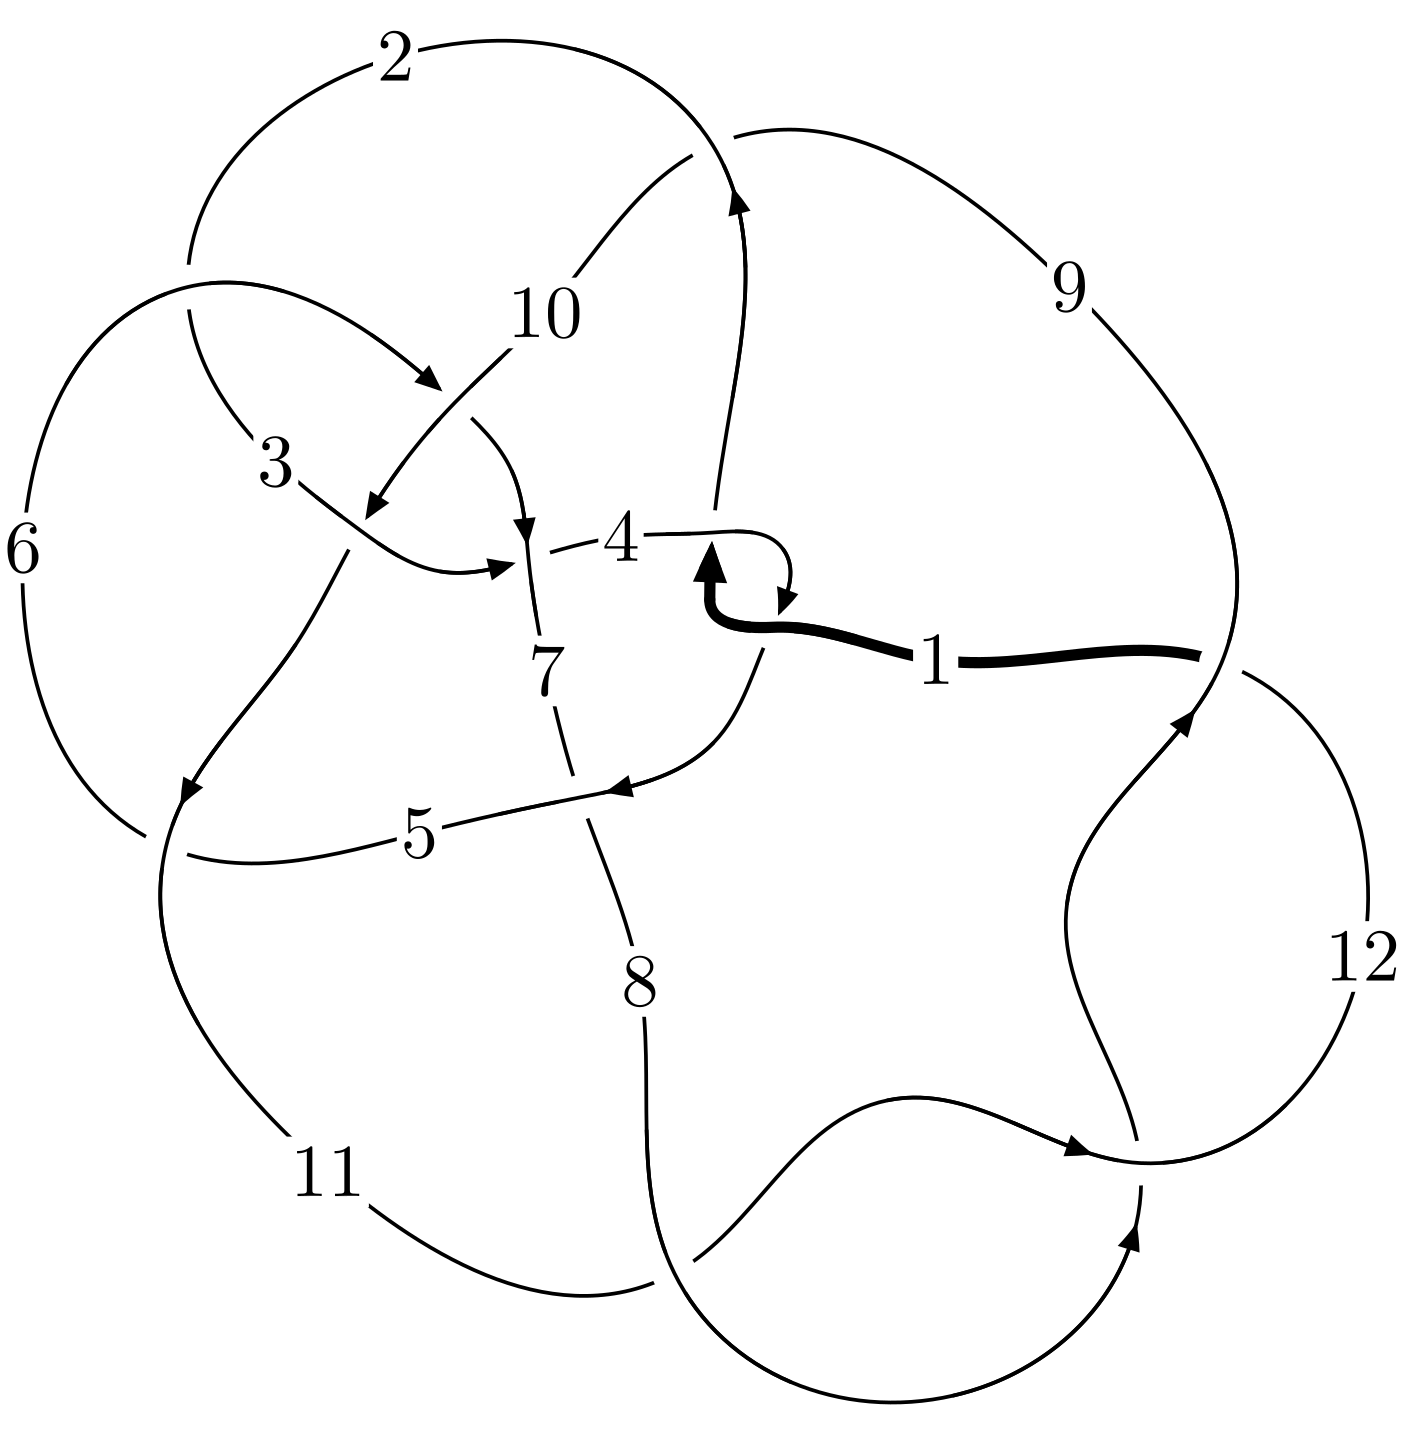
\includegraphics[width=112pt]{../../../GIT/diagram.site/Diagrams/png/1692_12a_0891.png}\\
\ \ \ A knot diagram\footnotemark}&
\allowdisplaybreaks
\textbf{Linearized knot diagam} \\
\cline{2-2}
 &
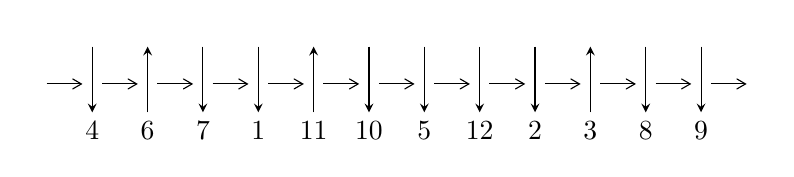
\begin{tikzpicture}[x=20pt, y=17pt]
	% nodes
	\node (C0) at (0, 0) {};
	\node (C1) at (1, 0) {};
	\node (C1U) at (1, +1) {};
	\node (C1D) at (1, -1) {4};

	\node (C2) at (2, 0) {};
	\node (C2U) at (2, +1) {};
	\node (C2D) at (2, -1) {6};

	\node (C3) at (3, 0) {};
	\node (C3U) at (3, +1) {};
	\node (C3D) at (3, -1) {7};

	\node (C4) at (4, 0) {};
	\node (C4U) at (4, +1) {};
	\node (C4D) at (4, -1) {1};

	\node (C5) at (5, 0) {};
	\node (C5U) at (5, +1) {};
	\node (C5D) at (5, -1) {11};

	\node (C6) at (6, 0) {};
	\node (C6U) at (6, +1) {};
	\node (C6D) at (6, -1) {10};

	\node (C7) at (7, 0) {};
	\node (C7U) at (7, +1) {};
	\node (C7D) at (7, -1) {5};

	\node (C8) at (8, 0) {};
	\node (C8U) at (8, +1) {};
	\node (C8D) at (8, -1) {12};

	\node (C9) at (9, 0) {};
	\node (C9U) at (9, +1) {};
	\node (C9D) at (9, -1) {2};

	\node (C10) at (10, 0) {};
	\node (C10U) at (10, +1) {};
	\node (C10D) at (10, -1) {3};

	\node (C11) at (11, 0) {};
	\node (C11U) at (11, +1) {};
	\node (C11D) at (11, -1) {8};

	\node (C12) at (12, 0) {};
	\node (C12U) at (12, +1) {};
	\node (C12D) at (12, -1) {9};
	\node (C13) at (13, 0) {};

	% arrows
	\draw[->,>={angle 60}]
	(C0) edge (C1) (C1) edge (C2) (C2) edge (C3) (C3) edge (C4) (C4) edge (C5) (C5) edge (C6) (C6) edge (C7) (C7) edge (C8) (C8) edge (C9) (C9) edge (C10) (C10) edge (C11) (C11) edge (C12) (C12) edge (C13) ;	\draw[->,>=stealth]
	(C1U) edge (C1D) (C2D) edge (C2U) (C3U) edge (C3D) (C4U) edge (C4D) (C5D) edge (C5U) (C6U) edge (C6D) (C7U) edge (C7D) (C8U) edge (C8D) (C9U) edge (C9D) (C10D) edge (C10U) (C11U) edge (C11D) (C12U) edge (C12D) ;
	\end{tikzpicture} \\
\hhline{~~} \\& 
\textbf{Solving Sequence} \\ \cline{2-2} 
 &
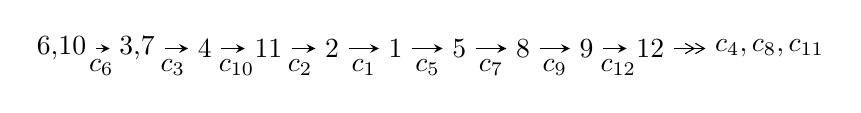
\begin{tikzpicture}[x=23pt, y=7pt]
	% node
	\node (A0) at (-1/8, 0) {6,10};
	\node (A1) at (17/16, 0) {3,7};
	\node (A2) at (17/8, 0) {4};
	\node (A3) at (25/8, 0) {11};
	\node (A4) at (33/8, 0) {2};
	\node (A5) at (41/8, 0) {1};
	\node (A6) at (49/8, 0) {5};
	\node (A7) at (57/8, 0) {8};
	\node (A8) at (65/8, 0) {9};
	\node (A9) at (73/8, 0) {12};
	\node (C1) at (1/2, -1) {$c_{6}$};
	\node (C2) at (13/8, -1) {$c_{3}$};
	\node (C3) at (21/8, -1) {$c_{10}$};
	\node (C4) at (29/8, -1) {$c_{2}$};
	\node (C5) at (37/8, -1) {$c_{1}$};
	\node (C6) at (45/8, -1) {$c_{5}$};
	\node (C7) at (53/8, -1) {$c_{7}$};
	\node (C8) at (61/8, -1) {$c_{9}$};
	\node (C9) at (69/8, -1) {$c_{12}$};
	\node (A10) at (11, 0) {$c_{4},c_{8},c_{11}$};

	% edge
	\draw[->,>=stealth]	
	(A0) edge (A1) (A1) edge (A2) (A2) edge (A3) (A3) edge (A4) (A4) edge (A5) (A5) edge (A6) (A6) edge (A7) (A7) edge (A8) (A8) edge (A9) ;
	\draw[->>,>={angle 60}]	
	(A9) edge (A10);
\end{tikzpicture} \\ 

\end{tabular} \\

\footnotetext{
The image of knot diagram is generated by the software ``\textbf{Draw programme}" developed by Andrew Bartholomew(\url{http://www.layer8.co.uk/maths/draw/index.htm\#Running-draw}), where we modified some parts for our purpose(\url{https://github.com/CATsTAILs/LinksPainter}).
}\phantom \\ \newline 
\centering \textbf{Ideals for irreducible components\footnotemark of $X_{\text{par}}$} 
 
\begin{align*}
I^u_{1}&=\langle 
3.11585\times10^{1116} u^{152}+1.63261\times10^{1116} u^{151}+\cdots+7.00851\times10^{1115} b-6.18169\times10^{1116},\\
\phantom{I^u_{1}}&\phantom{= \langle  }3.79481\times10^{1116} u^{152}+2.05132\times10^{1116} u^{151}+\cdots+7.00851\times10^{1115} a-9.83526\times10^{1116},\\
\phantom{I^u_{1}}&\phantom{= \langle  }u^{153}+u^{152}+\cdots-3 u-1\rangle \\
I^u_{2}&=\langle 
-2.36234\times10^{27} u^{30}-5.41386\times10^{27} u^{29}+\cdots+6.33336\times10^{27} b-9.12988\times10^{27},\\
\phantom{I^u_{2}}&\phantom{= \langle  }2.80253\times10^{27} u^{30}+5.27117\times10^{27} u^{29}+\cdots+6.33336\times10^{27} a+1.02266\times10^{28},\;u^{31}+3 u^{30}+\cdots+u+1\rangle \\
I^u_{3}&=\langle 
b,\;- u^5+2 u^4+4 u^3-9 u^2+4 a+13 u-5,\;u^6-3 u^5+2 u^4-3 u^3-2 u^2-2 u-1\rangle \\
\\
\end{align*}
\raggedright * 3 irreducible components of $\dim_{\mathbb{C}}=0$, with total 190 representations.\\
\footnotetext{All coefficients of polynomials are rational numbers. But the coefficients are sometimes approximated in decimal forms when there is not enough margin.}
\newpage
\renewcommand{\arraystretch}{1}
\centering \section*{I. $I^u_{1}= \langle 3.12\times10^{1116} u^{152}+1.63\times10^{1116} u^{151}+\cdots+7.01\times10^{1115} b-6.18\times10^{1116},\;3.79\times10^{1116} u^{152}+2.05\times10^{1116} u^{151}+\cdots+7.01\times10^{1115} a-9.84\times10^{1116},\;u^{153}+u^{152}+\cdots-3 u-1 \rangle$}
\flushleft \textbf{(i) Arc colorings}\\
\begin{tabular}{m{7pt} m{180pt} m{7pt} m{180pt} }
\flushright $a_{6}=$&$\begin{pmatrix}1\\0\end{pmatrix}$ \\
\flushright $a_{10}=$&$\begin{pmatrix}0\\u\end{pmatrix}$ \\
\flushright $a_{3}=$&$\begin{pmatrix}-5.41457 u^{152}-2.92690 u^{151}+\cdots-14.9314 u+14.0333\\-4.44582 u^{152}-2.32946 u^{151}+\cdots+5.48619 u+8.82027\end{pmatrix}$ \\
\flushright $a_{7}=$&$\begin{pmatrix}1\\u^2\end{pmatrix}$ \\
\flushright $a_{4}=$&$\begin{pmatrix}-2.16296 u^{152}-1.21387 u^{151}+\cdots-18.3691 u+7.70073\\-3.81062 u^{152}-1.86944 u^{151}+\cdots+4.12205 u+7.28169\end{pmatrix}$ \\
\flushright $a_{11}=$&$\begin{pmatrix}1.57210 u^{152}+1.32824 u^{151}+\cdots+44.1822 u-6.53834\\-1.94193 u^{152}-0.485705 u^{151}+\cdots+6.20185 u+1.74833\end{pmatrix}$ \\
\flushright $a_{2}=$&$\begin{pmatrix}-0.968757 u^{152}-0.597437 u^{151}+\cdots-20.4176 u+5.21305\\-4.44582 u^{152}-2.32946 u^{151}+\cdots+5.48619 u+8.82027\end{pmatrix}$ \\
\flushright $a_{1}=$&$\begin{pmatrix}1.66932 u^{152}+0.497431 u^{151}+\cdots-23.0859 u+2.01272\\-2.13293 u^{152}-1.01455 u^{151}+\cdots-1.93762 u+4.02211\end{pmatrix}$ \\
\flushright $a_{5}=$&$\begin{pmatrix}-3.61369 u^{152}-1.21232 u^{151}+\cdots-22.2380 u+11.3427\\-3.40152 u^{152}-1.28917 u^{151}+\cdots+1.85705 u+5.98673\end{pmatrix}$ \\
\flushright $a_{8}=$&$\begin{pmatrix}-5.90920 u^{152}-3.75096 u^{151}+\cdots-12.6563 u+14.0426\\4.60273 u^{152}+1.50922 u^{151}+\cdots-11.8883 u-5.78819\end{pmatrix}$ \\
\flushright $a_{9}=$&$\begin{pmatrix}-0.342166 u^{152}+0.639353 u^{151}+\cdots+48.2398 u-2.78180\\3.85620 u^{152}+1.17459 u^{151}+\cdots-8.25942 u-5.50487\end{pmatrix}$ \\
\flushright $a_{12}=$&$\begin{pmatrix}2.29977 u^{152}+1.43257 u^{151}+\cdots+9.44943 u-1.68228\\5.25264 u^{152}+1.44816 u^{151}+\cdots-12.5949 u-7.66935\end{pmatrix}$\\&\end{tabular}
\flushleft \textbf{(ii) Obstruction class $= -1$}\\~\\
\flushleft \textbf{(iii) Cusp Shapes $= 0.951754 u^{152}-2.70912 u^{151}+\cdots-13.7606 u+0.254180$}\\~\\
\newpage\renewcommand{\arraystretch}{1}
\flushleft \textbf{(iv) u-Polynomials at the component}\newline \\
\begin{tabular}{m{50pt}|m{274pt}}
Crossings & \hspace{64pt}u-Polynomials at each crossing \\
\hline $$\begin{aligned}c_{1},c_{4}\end{aligned}$$&$\begin{aligned}
&u^{153}+6 u^{152}+\cdots-839 u-307
\end{aligned}$\\
\hline $$\begin{aligned}c_{2}\end{aligned}$$&$\begin{aligned}
&u^{153}-8 u^{152}+\cdots-1344 u-64
\end{aligned}$\\
\hline $$\begin{aligned}c_{3}\end{aligned}$$&$\begin{aligned}
&u^{153}- u^{152}+\cdots+615240 u-163556
\end{aligned}$\\
\hline $$\begin{aligned}c_{5}\end{aligned}$$&$\begin{aligned}
&u^{153}+42 u^{151}+\cdots-56802438868 u-10797888812
\end{aligned}$\\
\hline $$\begin{aligned}c_{6}\end{aligned}$$&$\begin{aligned}
&u^{153}+u^{152}+\cdots-3 u-1
\end{aligned}$\\
\hline $$\begin{aligned}c_{7}\end{aligned}$$&$\begin{aligned}
&u^{153}+5 u^{152}+\cdots-2075740 u-194200
\end{aligned}$\\
\hline $$\begin{aligned}c_{8},c_{11},c_{12}\end{aligned}$$&$\begin{aligned}
&u^{153}-77 u^{151}+\cdots+13 u-1
\end{aligned}$\\
\hline $$\begin{aligned}c_{9}\end{aligned}$$&$\begin{aligned}
&u^{153}-33 u^{151}+\cdots+680974452 u-75062943
\end{aligned}$\\
\hline $$\begin{aligned}c_{10}\end{aligned}$$&$\begin{aligned}
&u^{153}+4 u^{152}+\cdots+17 u+1
\end{aligned}$\\
\hline
\end{tabular}\\~\\
\newpage\renewcommand{\arraystretch}{1}
\flushleft \textbf{(v) Riley Polynomials at the component}\newline \\
\begin{tabular}{m{50pt}|m{274pt}}
Crossings & \hspace{64pt}Riley Polynomials at each crossing \\
\hline $$\begin{aligned}c_{1},c_{4}\end{aligned}$$&$\begin{aligned}
&y^{153}+92 y^{152}+\cdots-3754947 y-94249
\end{aligned}$\\
\hline $$\begin{aligned}c_{2}\end{aligned}$$&$\begin{aligned}
&y^{153}+44 y^{152}+\cdots+1161216 y-4096
\end{aligned}$\\
\hline $$\begin{aligned}c_{3}\end{aligned}$$&$\begin{aligned}
&y^{153}-21 y^{152}+\cdots+1454894069632 y-26750565136
\end{aligned}$\\
\hline $$\begin{aligned}c_{5}\end{aligned}$$&$\begin{aligned}
&y^{153}+84 y^{152}+\cdots-5.53\times10^{21} y-1.17\times10^{20}
\end{aligned}$\\
\hline $$\begin{aligned}c_{6}\end{aligned}$$&$\begin{aligned}
&y^{153}-21 y^{152}+\cdots+73 y-1
\end{aligned}$\\
\hline $$\begin{aligned}c_{7}\end{aligned}$$&$\begin{aligned}
&y^{153}-47 y^{152}+\cdots+2201363212400 y-37713640000
\end{aligned}$\\
\hline $$\begin{aligned}c_{8},c_{11},c_{12}\end{aligned}$$&$\begin{aligned}
&y^{153}-154 y^{152}+\cdots+y-1
\end{aligned}$\\
\hline $$\begin{aligned}c_{9}\end{aligned}$$&$\begin{aligned}
&y^{153}-66 y^{152}+\cdots+487511585631586602 y-5634445411821249
\end{aligned}$\\
\hline $$\begin{aligned}c_{10}\end{aligned}$$&$\begin{aligned}
&y^{153}+24 y^{152}+\cdots-555 y-1
\end{aligned}$\\
\hline
\end{tabular}\\~\\
\newpage\flushleft \textbf{(vi) Complex Volumes and Cusp Shapes}
$$\begin{array}{c|c|c}  
\text{Solutions to }I^u_{1}& \I (\text{vol} + \sqrt{-1}CS) & \text{Cusp shape}\\
 \hline 
\begin{aligned}
u &= \phantom{-}0.973353 + 0.148533 I \\
a &= -1.04719 + 1.41780 I \\
b &= -0.417717 + 0.750536 I\end{aligned}
 & -8.58768 - 7.55812 I & \phantom{-0.000000 } 0 \\ \hline\begin{aligned}
u &= \phantom{-}0.973353 - 0.148533 I \\
a &= -1.04719 - 1.41780 I \\
b &= -0.417717 - 0.750536 I\end{aligned}
 & -8.58768 + 7.55812 I & \phantom{-0.000000 } 0 \\ \hline\begin{aligned}
u &= \phantom{-}0.867373 + 0.453722 I \\
a &= \phantom{-}0.149660 - 0.797153 I \\
b &= \phantom{-}1.20531 - 1.58661 I\end{aligned}
 & -9.06733 - 5.39501 I & \phantom{-0.000000 } 0 \\ \hline\begin{aligned}
u &= \phantom{-}0.867373 - 0.453722 I \\
a &= \phantom{-}0.149660 + 0.797153 I \\
b &= \phantom{-}1.20531 + 1.58661 I\end{aligned}
 & -9.06733 + 5.39501 I & \phantom{-0.000000 } 0 \\ \hline\begin{aligned}
u &= -0.972730\phantom{ +0.000000I} \\
a &= \phantom{-}0.518545\phantom{ +0.000000I} \\
b &= -0.217110\phantom{ +0.000000I}\end{aligned}
 & -1.29206\phantom{ +0.000000I} & \phantom{-0.000000 } 0 \\ \hline\begin{aligned}
u &= \phantom{-}0.781124 + 0.577758 I \\
a &= \phantom{-}0.08294 - 1.58923 I \\
b &= \phantom{-}0.95531 - 1.16559 I\end{aligned}
 & \phantom{-}1.27140 - 4.48962 I & \phantom{-0.000000 } 0 \\ \hline\begin{aligned}
u &= \phantom{-}0.781124 - 0.577758 I \\
a &= \phantom{-}0.08294 + 1.58923 I \\
b &= \phantom{-}0.95531 + 1.16559 I\end{aligned}
 & \phantom{-}1.27140 + 4.48962 I & \phantom{-0.000000 } 0 \\ \hline\begin{aligned}
u &= -0.826284 + 0.494731 I \\
a &= \phantom{-}0.21183 + 1.66604 I \\
b &= \phantom{-}0.97788 + 1.47738 I\end{aligned}
 & -3.47461 + 5.28528 I & \phantom{-0.000000 } 0 \\ \hline\begin{aligned}
u &= -0.826284 - 0.494731 I \\
a &= \phantom{-}0.21183 - 1.66604 I \\
b &= \phantom{-}0.97788 - 1.47738 I\end{aligned}
 & -3.47461 - 5.28528 I & \phantom{-0.000000 } 0 \\ \hline\begin{aligned}
u &= \phantom{-}0.619722 + 0.736392 I \\
a &= \phantom{-}0.004500 - 0.337299 I \\
b &= \phantom{-}1.30690 - 0.66973 I\end{aligned}
 & -2.45600 - 5.85568 I & \phantom{-0.000000 } 0\\
 \hline 
 \end{array}$$\newpage$$\begin{array}{c|c|c}  
\text{Solutions to }I^u_{1}& \I (\text{vol} + \sqrt{-1}CS) & \text{Cusp shape}\\
 \hline 
\begin{aligned}
u &= \phantom{-}0.619722 - 0.736392 I \\
a &= \phantom{-}0.004500 + 0.337299 I \\
b &= \phantom{-}1.30690 + 0.66973 I\end{aligned}
 & -2.45600 + 5.85568 I & \phantom{-0.000000 } 0 \\ \hline\begin{aligned}
u &= -0.329800 + 0.898354 I \\
a &= \phantom{-}0.249134 - 1.285850 I \\
b &= -0.0813293 + 0.0031954 I\end{aligned}
 & \phantom{-}2.99162 + 2.89965 I & \phantom{-0.000000 } 0 \\ \hline\begin{aligned}
u &= -0.329800 - 0.898354 I \\
a &= \phantom{-}0.249134 + 1.285850 I \\
b &= -0.0813293 - 0.0031954 I\end{aligned}
 & \phantom{-}2.99162 - 2.89965 I & \phantom{-0.000000 } 0 \\ \hline\begin{aligned}
u &= \phantom{-}0.356418 + 0.985409 I \\
a &= \phantom{-}0.434742 + 1.241200 I \\
b &= -0.443127 - 0.087929 I\end{aligned}
 & -2.26925 - 3.85824 I & \phantom{-0.000000 } 0 \\ \hline\begin{aligned}
u &= \phantom{-}0.356418 - 0.985409 I \\
a &= \phantom{-}0.434742 - 1.241200 I \\
b &= -0.443127 + 0.087929 I\end{aligned}
 & -2.26925 + 3.85824 I & \phantom{-0.000000 } 0 \\ \hline\begin{aligned}
u &= \phantom{-}1.05005\phantom{ +0.000000I} \\
a &= -0.0880587\phantom{ +0.000000I} \\
b &= -1.15611\phantom{ +0.000000I}\end{aligned}
 & -6.56914\phantom{ +0.000000I} & \phantom{-0.000000 } 0 \\ \hline\begin{aligned}
u &= -0.393235 + 0.857642 I \\
a &= -1.06688 + 1.48421 I \\
b &= \phantom{-}0.901301 + 0.488346 I\end{aligned}
 & \phantom{-}2.61679 + 6.43034 I & \phantom{-0.000000 } 0 \\ \hline\begin{aligned}
u &= -0.393235 - 0.857642 I \\
a &= -1.06688 - 1.48421 I \\
b &= \phantom{-}0.901301 - 0.488346 I\end{aligned}
 & \phantom{-}2.61679 - 6.43034 I & \phantom{-0.000000 } 0 \\ \hline\begin{aligned}
u &= -0.895296 + 0.589714 I \\
a &= \phantom{-}0.310160 + 1.325900 I \\
b &= \phantom{-}1.19061 + 0.94394 I\end{aligned}
 & -2.74813 + 3.64489 I & \phantom{-0.000000 } 0 \\ \hline\begin{aligned}
u &= -0.895296 - 0.589714 I \\
a &= \phantom{-}0.310160 - 1.325900 I \\
b &= \phantom{-}1.19061 - 0.94394 I\end{aligned}
 & -2.74813 - 3.64489 I & \phantom{-0.000000 } 0\\
 \hline 
 \end{array}$$\newpage$$\begin{array}{c|c|c}  
\text{Solutions to }I^u_{1}& \I (\text{vol} + \sqrt{-1}CS) & \text{Cusp shape}\\
 \hline 
\begin{aligned}
u &= \phantom{-}0.795571 + 0.473574 I \\
a &= \phantom{-}1.59964 - 0.10837 I \\
b &= \phantom{-}0.066361 + 0.614898 I\end{aligned}
 & -9.04738 + 1.18227 I & \phantom{-0.000000 } 0 \\ \hline\begin{aligned}
u &= \phantom{-}0.795571 - 0.473574 I \\
a &= \phantom{-}1.59964 + 0.10837 I \\
b &= \phantom{-}0.066361 - 0.614898 I\end{aligned}
 & -9.04738 - 1.18227 I & \phantom{-0.000000 } 0 \\ \hline\begin{aligned}
u &= -0.812516 + 0.439182 I \\
a &= -0.245879 + 0.500905 I \\
b &= -0.893866 + 0.708689 I\end{aligned}
 & -2.09655 + 0.26711 I & \phantom{-0.000000 } 0 \\ \hline\begin{aligned}
u &= -0.812516 - 0.439182 I \\
a &= -0.245879 - 0.500905 I \\
b &= -0.893866 - 0.708689 I\end{aligned}
 & -2.09655 - 0.26711 I & \phantom{-0.000000 } 0 \\ \hline\begin{aligned}
u &= -0.421496 + 0.992141 I \\
a &= \phantom{-}0.068442 + 0.960075 I \\
b &= \phantom{-}0.23495 + 1.81386 I\end{aligned}
 & \phantom{-}0.86232 + 2.51923 I & \phantom{-0.000000 } 0 \\ \hline\begin{aligned}
u &= -0.421496 - 0.992141 I \\
a &= \phantom{-}0.068442 - 0.960075 I \\
b &= \phantom{-}0.23495 - 1.81386 I\end{aligned}
 & \phantom{-}0.86232 - 2.51923 I & \phantom{-0.000000 } 0 \\ \hline\begin{aligned}
u &= -0.061438 + 0.902325 I \\
a &= \phantom{-}0.075783 - 1.027940 I \\
b &= -0.44341 - 1.89241 I\end{aligned}
 & \phantom{-}2.02051 + 4.84345 I & \phantom{-0.000000 } 0 \\ \hline\begin{aligned}
u &= -0.061438 - 0.902325 I \\
a &= \phantom{-}0.075783 + 1.027940 I \\
b &= -0.44341 + 1.89241 I\end{aligned}
 & \phantom{-}2.02051 - 4.84345 I & \phantom{-0.000000 } 0 \\ \hline\begin{aligned}
u &= -0.833519 + 0.344884 I \\
a &= \phantom{-}0.143031 + 0.852046 I \\
b &= \phantom{-}0.97507 + 1.20612 I\end{aligned}
 & -1.60976 + 3.75013 I & \phantom{-0.000000 } 0 \\ \hline\begin{aligned}
u &= -0.833519 - 0.344884 I \\
a &= \phantom{-}0.143031 - 0.852046 I \\
b &= \phantom{-}0.97507 - 1.20612 I\end{aligned}
 & -1.60976 - 3.75013 I & \phantom{-0.000000 } 0\\
 \hline 
 \end{array}$$\newpage$$\begin{array}{c|c|c}  
\text{Solutions to }I^u_{1}& \I (\text{vol} + \sqrt{-1}CS) & \text{Cusp shape}\\
 \hline 
\begin{aligned}
u &= \phantom{-}0.201392 + 0.878936 I \\
a &= \phantom{-}0.25333 + 1.48149 I \\
b &= \phantom{-}0.156786 - 0.309665 I\end{aligned}
 & -1.19863 - 2.66458 I & \phantom{-0.000000 } 0 \\ \hline\begin{aligned}
u &= \phantom{-}0.201392 - 0.878936 I \\
a &= \phantom{-}0.25333 - 1.48149 I \\
b &= \phantom{-}0.156786 + 0.309665 I\end{aligned}
 & -1.19863 + 2.66458 I & \phantom{-0.000000 } 0 \\ \hline\begin{aligned}
u &= -0.527832 + 0.993727 I \\
a &= \phantom{-}0.082403 - 1.023070 I \\
b &= -0.468349 - 0.777321 I\end{aligned}
 & \phantom{-}3.84410 + 4.00937 I & \phantom{-0.000000 } 0 \\ \hline\begin{aligned}
u &= -0.527832 - 0.993727 I \\
a &= \phantom{-}0.082403 + 1.023070 I \\
b &= -0.468349 + 0.777321 I\end{aligned}
 & \phantom{-}3.84410 - 4.00937 I & \phantom{-0.000000 } 0 \\ \hline\begin{aligned}
u &= \phantom{-}0.497291 + 1.036640 I \\
a &= \phantom{-}0.088921 + 0.906155 I \\
b &= -0.791615 + 0.502372 I\end{aligned}
 & \phantom{-}5.64479 + 0.25144 I & \phantom{-0.000000 } 0 \\ \hline\begin{aligned}
u &= \phantom{-}0.497291 - 1.036640 I \\
a &= \phantom{-}0.088921 - 0.906155 I \\
b &= -0.791615 - 0.502372 I\end{aligned}
 & \phantom{-}5.64479 - 0.25144 I & \phantom{-0.000000 } 0 \\ \hline\begin{aligned}
u &= \phantom{-}0.405116 + 1.080960 I \\
a &= -1.01082 - 1.00751 I \\
b &= \phantom{-}1.188840 - 0.415562 I\end{aligned}
 & -3.17421 - 9.26039 I & \phantom{-0.000000 } 0 \\ \hline\begin{aligned}
u &= \phantom{-}0.405116 - 1.080960 I \\
a &= -1.01082 + 1.00751 I \\
b &= \phantom{-}1.188840 + 0.415562 I\end{aligned}
 & -3.17421 + 9.26039 I & \phantom{-0.000000 } 0 \\ \hline\begin{aligned}
u &= -0.781644 + 0.300193 I \\
a &= \phantom{-}1.77937 - 0.79388 I \\
b &= -0.060681 - 0.552079 I\end{aligned}
 & -1.49841 + 1.51843 I & \phantom{-0.000000 } 0 \\ \hline\begin{aligned}
u &= -0.781644 - 0.300193 I \\
a &= \phantom{-}1.77937 + 0.79388 I \\
b &= -0.060681 + 0.552079 I\end{aligned}
 & -1.49841 - 1.51843 I & \phantom{-0.000000 } 0\\
 \hline 
 \end{array}$$\newpage$$\begin{array}{c|c|c}  
\text{Solutions to }I^u_{1}& \I (\text{vol} + \sqrt{-1}CS) & \text{Cusp shape}\\
 \hline 
\begin{aligned}
u &= -0.554491 + 1.042730 I \\
a &= \phantom{-}0.239454 - 0.192604 I \\
b &= \phantom{-}0.335302 - 1.053270 I\end{aligned}
 & -0.18119 + 2.07511 I & \phantom{-0.000000 } 0 \\ \hline\begin{aligned}
u &= -0.554491 - 1.042730 I \\
a &= \phantom{-}0.239454 + 0.192604 I \\
b &= \phantom{-}0.335302 + 1.053270 I\end{aligned}
 & -0.18119 - 2.07511 I & \phantom{-0.000000 } 0 \\ \hline\begin{aligned}
u &= -0.773515 + 0.268831 I \\
a &= -0.80494 - 2.04805 I \\
b &= -0.341865 - 0.645055 I\end{aligned}
 & -2.80427 + 3.49940 I & \phantom{-0.000000 } 0 \\ \hline\begin{aligned}
u &= -0.773515 - 0.268831 I \\
a &= -0.80494 + 2.04805 I \\
b &= -0.341865 + 0.645055 I\end{aligned}
 & -2.80427 - 3.49940 I & \phantom{-0.000000 } 0 \\ \hline\begin{aligned}
u &= \phantom{-}1.100940 + 0.450679 I \\
a &= -0.293571 - 0.397214 I \\
b &= -1.07149 - 0.97058 I\end{aligned}
 & -7.11145 + 0.23787 I & \phantom{-0.000000 } 0 \\ \hline\begin{aligned}
u &= \phantom{-}1.100940 - 0.450679 I \\
a &= -0.293571 + 0.397214 I \\
b &= -1.07149 + 0.97058 I\end{aligned}
 & -7.11145 - 0.23787 I & \phantom{-0.000000 } 0 \\ \hline\begin{aligned}
u &= \phantom{-}0.318683 + 0.730046 I \\
a &= \phantom{-}0.055493 + 1.093020 I \\
b &= -1.07179 + 1.87224 I\end{aligned}
 & -5.05861 - 10.12750 I & \phantom{-0.000000 } 0 \\ \hline\begin{aligned}
u &= \phantom{-}0.318683 - 0.730046 I \\
a &= \phantom{-}0.055493 - 1.093020 I \\
b &= -1.07179 - 1.87224 I\end{aligned}
 & -5.05861 + 10.12750 I & \phantom{-0.000000 } 0 \\ \hline\begin{aligned}
u &= -0.504370 + 1.100750 I \\
a &= \phantom{-}0.055033 - 0.790183 I \\
b &= -0.930533 - 0.292260 I\end{aligned}
 & \phantom{-}0.11426 - 3.67355 I & \phantom{-0.000000 } 0 \\ \hline\begin{aligned}
u &= -0.504370 - 1.100750 I \\
a &= \phantom{-}0.055033 + 0.790183 I \\
b &= -0.930533 + 0.292260 I\end{aligned}
 & \phantom{-}0.11426 + 3.67355 I & \phantom{-0.000000 } 0\\
 \hline 
 \end{array}$$\newpage$$\begin{array}{c|c|c}  
\text{Solutions to }I^u_{1}& \I (\text{vol} + \sqrt{-1}CS) & \text{Cusp shape}\\
 \hline 
\begin{aligned}
u &= -0.683605 + 0.383090 I \\
a &= \phantom{-}0.835310 - 0.266566 I \\
b &= -0.083301 - 0.373260 I\end{aligned}
 & -1.220670 + 0.364289 I & \phantom{-0.000000 } 0 \\ \hline\begin{aligned}
u &= -0.683605 - 0.383090 I \\
a &= \phantom{-}0.835310 + 0.266566 I \\
b &= -0.083301 + 0.373260 I\end{aligned}
 & -1.220670 - 0.364289 I & \phantom{-0.000000 } 0 \\ \hline\begin{aligned}
u &= -0.186368 + 0.743142 I \\
a &= \phantom{-}0.0714649 - 0.0048705 I \\
b &= \phantom{-}1.17367 + 0.86749 I\end{aligned}
 & \phantom{-}2.17358 + 2.56779 I & \phantom{-0.000000 } 0 \\ \hline\begin{aligned}
u &= -0.186368 - 0.743142 I \\
a &= \phantom{-}0.0714649 + 0.0048705 I \\
b &= \phantom{-}1.17367 - 0.86749 I\end{aligned}
 & \phantom{-}2.17358 - 2.56779 I & \phantom{-0.000000 } 0 \\ \hline\begin{aligned}
u &= -0.702889 + 0.206928 I \\
a &= \phantom{-}0.43730 + 1.59440 I \\
b &= -0.08565 + 1.60880 I\end{aligned}
 & -6.00659 + 5.00728 I & \phantom{-0.000000 } 0 \\ \hline\begin{aligned}
u &= -0.702889 - 0.206928 I \\
a &= \phantom{-}0.43730 - 1.59440 I \\
b &= -0.08565 - 1.60880 I\end{aligned}
 & -6.00659 - 5.00728 I & \phantom{-0.000000 } 0 \\ \hline\begin{aligned}
u &= \phantom{-}1.157010 + 0.567669 I \\
a &= \phantom{-}0.348684 - 0.730841 I \\
b &= \phantom{-}0.820526 - 0.685310 I\end{aligned}
 & \phantom{-}0.56887 - 2.07115 I & \phantom{-0.000000 } 0 \\ \hline\begin{aligned}
u &= \phantom{-}1.157010 - 0.567669 I \\
a &= \phantom{-}0.348684 + 0.730841 I \\
b &= \phantom{-}0.820526 + 0.685310 I\end{aligned}
 & \phantom{-}0.56887 + 2.07115 I & \phantom{-0.000000 } 0 \\ \hline\begin{aligned}
u &= \phantom{-}0.631950 + 0.294444 I \\
a &= \phantom{-}2.70218 + 0.77459 I \\
b &= -0.157887 + 0.567601 I\end{aligned}
 & -0.58566 - 6.76292 I & \phantom{-0.000000 } 0 \\ \hline\begin{aligned}
u &= \phantom{-}0.631950 - 0.294444 I \\
a &= \phantom{-}2.70218 - 0.77459 I \\
b &= -0.157887 - 0.567601 I\end{aligned}
 & -0.58566 + 6.76292 I & \phantom{-0.000000 } 0\\
 \hline 
 \end{array}$$\newpage$$\begin{array}{c|c|c}  
\text{Solutions to }I^u_{1}& \I (\text{vol} + \sqrt{-1}CS) & \text{Cusp shape}\\
 \hline 
\begin{aligned}
u &= -0.626657 + 0.252019 I \\
a &= \phantom{-}0.33296 + 1.82587 I \\
b &= \phantom{-}1.020000 + 0.826234 I\end{aligned}
 & -3.12725 + 3.37507 I & \phantom{-0.000000 } 0 \\ \hline\begin{aligned}
u &= -0.626657 - 0.252019 I \\
a &= \phantom{-}0.33296 - 1.82587 I \\
b &= \phantom{-}1.020000 - 0.826234 I\end{aligned}
 & -3.12725 - 3.37507 I & \phantom{-0.000000 } 0 \\ \hline\begin{aligned}
u &= -0.571915 + 0.353443 I \\
a &= \phantom{-}3.04284 - 0.26347 I \\
b &= -0.224004 - 0.635965 I\end{aligned}
 & -6.93504 + 10.92390 I & \phantom{-0.000000 } 0 \\ \hline\begin{aligned}
u &= -0.571915 - 0.353443 I \\
a &= \phantom{-}3.04284 + 0.26347 I \\
b &= -0.224004 + 0.635965 I\end{aligned}
 & -6.93504 - 10.92390 I & \phantom{-0.000000 } 0 \\ \hline\begin{aligned}
u &= -1.065600 + 0.804520 I \\
a &= -0.032315 + 0.873196 I \\
b &= \phantom{-}0.94789 + 1.10004 I\end{aligned}
 & -1.78649 + 4.39191 I & \phantom{-0.000000 } 0 \\ \hline\begin{aligned}
u &= -1.065600 - 0.804520 I \\
a &= -0.032315 - 0.873196 I \\
b &= \phantom{-}0.94789 - 1.10004 I\end{aligned}
 & -1.78649 - 4.39191 I & \phantom{-0.000000 } 0 \\ \hline\begin{aligned}
u &= -0.647944 + 0.052897 I \\
a &= -2.15693 + 2.10454 I \\
b &= -0.026201 + 0.892423 I\end{aligned}
 & -10.90870 + 3.66614 I & -22.9081 + 0. I\phantom{ +0.000000I} \\ \hline\begin{aligned}
u &= -0.647944 - 0.052897 I \\
a &= -2.15693 - 2.10454 I \\
b &= -0.026201 - 0.892423 I\end{aligned}
 & -10.90870 - 3.66614 I & -22.9081 + 0. I\phantom{ +0.000000I} \\ \hline\begin{aligned}
u &= \phantom{-}0.576304 + 0.297865 I \\
a &= -0.74284 - 1.53036 I \\
b &= \phantom{-}0.924640 - 0.897404 I\end{aligned}
 & \phantom{-}0.05784 - 3.70712 I & \phantom{-0.000000 } 0 \\ \hline\begin{aligned}
u &= \phantom{-}0.576304 - 0.297865 I \\
a &= -0.74284 + 1.53036 I \\
b &= \phantom{-}0.924640 + 0.897404 I\end{aligned}
 & \phantom{-}0.05784 + 3.70712 I & \phantom{-0.000000 } 0\\
 \hline 
 \end{array}$$\newpage$$\begin{array}{c|c|c}  
\text{Solutions to }I^u_{1}& \I (\text{vol} + \sqrt{-1}CS) & \text{Cusp shape}\\
 \hline 
\begin{aligned}
u &= -0.618264 + 0.173096 I \\
a &= \phantom{-}0.135414 - 0.910542 I \\
b &= \phantom{-}1.70579 - 1.69790 I\end{aligned}
 & -7.29185 + 10.11150 I & -18.4720 - 11.8238 I \\ \hline\begin{aligned}
u &= -0.618264 - 0.173096 I \\
a &= \phantom{-}0.135414 + 0.910542 I \\
b &= \phantom{-}1.70579 + 1.69790 I\end{aligned}
 & -7.29185 - 10.11150 I & -18.4720 + 11.8238 I \\ \hline\begin{aligned}
u &= -1.36448\phantom{ +0.000000I} \\
a &= \phantom{-}0.660395\phantom{ +0.000000I} \\
b &= \phantom{-}0.785262\phantom{ +0.000000I}\end{aligned}
 & -2.86005\phantom{ +0.000000I} & \phantom{-0.000000 } 0 \\ \hline\begin{aligned}
u &= \phantom{-}0.614991 + 0.133702 I \\
a &= \phantom{-}0.818152 - 1.102080 I \\
b &= \phantom{-}0.633098 - 0.666609 I\end{aligned}
 & \phantom{-}0.75866 - 1.62813 I & \phantom{-0.000000 -}0. + 3.46469 I \\ \hline\begin{aligned}
u &= \phantom{-}0.614991 - 0.133702 I \\
a &= \phantom{-}0.818152 + 1.102080 I \\
b &= \phantom{-}0.633098 + 0.666609 I\end{aligned}
 & \phantom{-}0.75866 + 1.62813 I & \phantom{-0.000000 } 0. - 3.46469 I \\ \hline\begin{aligned}
u &= \phantom{-}0.358121 + 0.510471 I \\
a &= -0.61433 - 2.94445 I \\
b &= \phantom{-}0.383855 - 0.598168 I\end{aligned}
 & \phantom{-}0.98655 - 3.25875 I & -6.00000 + 8.72783 I \\ \hline\begin{aligned}
u &= \phantom{-}0.358121 - 0.510471 I \\
a &= -0.61433 + 2.94445 I \\
b &= \phantom{-}0.383855 + 0.598168 I\end{aligned}
 & \phantom{-}0.98655 + 3.25875 I & -6.00000 - 8.72783 I \\ \hline\begin{aligned}
u &= \phantom{-}1.067710 + 0.878468 I \\
a &= -0.007537 + 1.111750 I \\
b &= -0.555437 + 1.288330 I\end{aligned}
 & -9.31337 - 0.97833 I & \phantom{-0.000000 } 0 \\ \hline\begin{aligned}
u &= \phantom{-}1.067710 - 0.878468 I \\
a &= -0.007537 - 1.111750 I \\
b &= -0.555437 - 1.288330 I\end{aligned}
 & -9.31337 + 0.97833 I & \phantom{-0.000000 } 0 \\ \hline\begin{aligned}
u &= -0.561932 + 0.251908 I \\
a &= -1.26889 + 2.08348 I \\
b &= \phantom{-}0.818448 + 1.013020 I\end{aligned}
 & -5.29787 + 5.09826 I & -17.0685 - 4.6385 I\\
 \hline 
 \end{array}$$\newpage$$\begin{array}{c|c|c}  
\text{Solutions to }I^u_{1}& \I (\text{vol} + \sqrt{-1}CS) & \text{Cusp shape}\\
 \hline 
\begin{aligned}
u &= -0.561932 - 0.251908 I \\
a &= -1.26889 - 2.08348 I \\
b &= \phantom{-}0.818448 - 1.013020 I\end{aligned}
 & -5.29787 - 5.09826 I & -17.0685 + 4.6385 I \\ \hline\begin{aligned}
u &= \phantom{-}0.591740 + 0.092087 I \\
a &= -1.74551 + 2.70376 I \\
b &= -0.093513 + 0.651902 I\end{aligned}
 & -3.81956 + 1.02043 I & -21.3279 + 0. I\phantom{ +0.000000I} \\ \hline\begin{aligned}
u &= \phantom{-}0.591740 - 0.092087 I \\
a &= -1.74551 - 2.70376 I \\
b &= -0.093513 - 0.651902 I\end{aligned}
 & -3.81956 - 1.02043 I & -21.3279 + 0. I\phantom{ +0.000000I} \\ \hline\begin{aligned}
u &= -0.589450 + 0.094016 I \\
a &= \phantom{-}0.083379 - 1.326010 I \\
b &= -1.39304 - 1.69778 I\end{aligned}
 & -10.65620 - 3.00835 I & -21.4885 + 0. I\phantom{ +0.000000I} \\ \hline\begin{aligned}
u &= -0.589450 - 0.094016 I \\
a &= \phantom{-}0.083379 + 1.326010 I \\
b &= -1.39304 + 1.69778 I\end{aligned}
 & -10.65620 + 3.00835 I & -21.4885 + 0. I\phantom{ +0.000000I} \\ \hline\begin{aligned}
u &= -1.092710 + 0.888260 I \\
a &= -0.007131 - 1.110860 I \\
b &= -0.727077 - 1.100620 I\end{aligned}
 & -3.44388 + 5.41506 I & \phantom{-0.000000 } 0 \\ \hline\begin{aligned}
u &= -1.092710 - 0.888260 I \\
a &= -0.007131 + 1.110860 I \\
b &= -0.727077 + 1.100620 I\end{aligned}
 & -3.44388 - 5.41506 I & \phantom{-0.000000 } 0 \\ \hline\begin{aligned}
u &= \phantom{-}1.19233 + 0.77344 I \\
a &= -0.228171 - 0.547479 I \\
b &= -0.232851 - 1.309320 I\end{aligned}
 & -8.26908 - 0.39568 I & \phantom{-0.000000 } 0 \\ \hline\begin{aligned}
u &= \phantom{-}1.19233 - 0.77344 I \\
a &= -0.228171 + 0.547479 I \\
b &= -0.232851 + 1.309320 I\end{aligned}
 & -8.26908 + 0.39568 I & \phantom{-0.000000 } 0 \\ \hline\begin{aligned}
u &= \phantom{-}0.476415 + 0.302223 I \\
a &= \phantom{-}0.045115 + 0.855413 I \\
b &= \phantom{-}1.79211 + 0.99841 I\end{aligned}
 & \phantom{-}0.16950 - 6.61987 I & -9.2353 + 17.8026 I\\
 \hline 
 \end{array}$$\newpage$$\begin{array}{c|c|c}  
\text{Solutions to }I^u_{1}& \I (\text{vol} + \sqrt{-1}CS) & \text{Cusp shape}\\
 \hline 
\begin{aligned}
u &= \phantom{-}0.476415 - 0.302223 I \\
a &= \phantom{-}0.045115 - 0.855413 I \\
b &= \phantom{-}1.79211 - 0.99841 I\end{aligned}
 & \phantom{-}0.16950 + 6.61987 I & -9.2353 - 17.8026 I \\ \hline\begin{aligned}
u &= -0.316116 + 0.461533 I \\
a &= -0.681920 - 0.916688 I \\
b &= \phantom{-}1.013040 + 0.132992 I\end{aligned}
 & \phantom{-}1.73851 + 2.42009 I & \phantom{-0.000000 } 0. - 4.60534 I \\ \hline\begin{aligned}
u &= -0.316116 - 0.461533 I \\
a &= -0.681920 + 0.916688 I \\
b &= \phantom{-}1.013040 - 0.132992 I\end{aligned}
 & \phantom{-}1.73851 - 2.42009 I & \phantom{-0.000000 -}0. + 4.60534 I \\ \hline\begin{aligned}
u &= -1.06891 + 0.97466 I \\
a &= -0.174523 + 0.372134 I \\
b &= -0.245761 + 0.682455 I\end{aligned}
 & -2.25355 + 0.65421 I & \phantom{-0.000000 } 0 \\ \hline\begin{aligned}
u &= -1.06891 - 0.97466 I \\
a &= -0.174523 - 0.372134 I \\
b &= -0.245761 - 0.682455 I\end{aligned}
 & -2.25355 - 0.65421 I & \phantom{-0.000000 } 0 \\ \hline\begin{aligned}
u &= \phantom{-}1.12825 + 0.90766 I \\
a &= -0.036226 + 1.071980 I \\
b &= -0.96360 + 1.15229 I\end{aligned}
 & -4.46458 - 9.83926 I & \phantom{-0.000000 } 0 \\ \hline\begin{aligned}
u &= \phantom{-}1.12825 - 0.90766 I \\
a &= -0.036226 - 1.071980 I \\
b &= -0.96360 - 1.15229 I\end{aligned}
 & -4.46458 + 9.83926 I & \phantom{-0.000000 } 0 \\ \hline\begin{aligned}
u &= -1.15321 + 0.88708 I \\
a &= -0.073268 - 1.097130 I \\
b &= -1.06186 - 1.27564 I\end{aligned}
 & -11.3463 + 12.7687 I & \phantom{-0.000000 } 0 \\ \hline\begin{aligned}
u &= -1.15321 - 0.88708 I \\
a &= -0.073268 + 1.097130 I \\
b &= -1.06186 + 1.27564 I\end{aligned}
 & -11.3463 - 12.7687 I & \phantom{-0.000000 } 0 \\ \hline\begin{aligned}
u &= \phantom{-}1.05683 + 1.00112 I \\
a &= -0.049387 - 0.910129 I \\
b &= \phantom{-}0.77650 - 1.48829 I\end{aligned}
 & -10.39940 - 5.61779 I & \phantom{-0.000000 } 0\\
 \hline 
 \end{array}$$\newpage$$\begin{array}{c|c|c}  
\text{Solutions to }I^u_{1}& \I (\text{vol} + \sqrt{-1}CS) & \text{Cusp shape}\\
 \hline 
\begin{aligned}
u &= \phantom{-}1.05683 - 1.00112 I \\
a &= -0.049387 + 0.910129 I \\
b &= \phantom{-}0.77650 + 1.48829 I\end{aligned}
 & -10.39940 + 5.61779 I & \phantom{-0.000000 } 0 \\ \hline\begin{aligned}
u &= \phantom{-}0.95068 + 1.10742 I \\
a &= \phantom{-}0.323524 + 1.009420 I \\
b &= -1.133040 + 0.823103 I\end{aligned}
 & -5.46544 - 7.07487 I & \phantom{-0.000000 } 0 \\ \hline\begin{aligned}
u &= \phantom{-}0.95068 - 1.10742 I \\
a &= \phantom{-}0.323524 - 1.009420 I \\
b &= -1.133040 - 0.823103 I\end{aligned}
 & -5.46544 + 7.07487 I & \phantom{-0.000000 } 0 \\ \hline\begin{aligned}
u &= \phantom{-}0.536184 + 0.052296 I \\
a &= -0.007625 - 1.229430 I \\
b &= -1.26962 - 1.20723 I\end{aligned}
 & -3.63573 - 1.60579 I & -22.7303 + 5.1459 I \\ \hline\begin{aligned}
u &= \phantom{-}0.536184 - 0.052296 I \\
a &= -0.007625 + 1.229430 I \\
b &= -1.26962 + 1.20723 I\end{aligned}
 & -3.63573 + 1.60579 I & -22.7303 - 5.1459 I \\ \hline\begin{aligned}
u &= \phantom{-}0.478861 + 0.215780 I \\
a &= \phantom{-}1.25793 - 1.91727 I \\
b &= -0.191534 - 1.031660 I\end{aligned}
 & \phantom{-}0.37950 - 3.31559 I & -10.26010 + 5.38518 I \\ \hline\begin{aligned}
u &= \phantom{-}0.478861 - 0.215780 I \\
a &= \phantom{-}1.25793 + 1.91727 I \\
b &= -0.191534 + 1.031660 I\end{aligned}
 & \phantom{-}0.37950 + 3.31559 I & -10.26010 - 5.38518 I \\ \hline\begin{aligned}
u &= \phantom{-}1.25844 + 0.86415 I \\
a &= -0.091391 - 0.703587 I \\
b &= \phantom{-}1.09013 - 1.47933 I\end{aligned}
 & -9.53310 - 5.23260 I & \phantom{-0.000000 } 0 \\ \hline\begin{aligned}
u &= \phantom{-}1.25844 - 0.86415 I \\
a &= -0.091391 + 0.703587 I \\
b &= \phantom{-}1.09013 + 1.47933 I\end{aligned}
 & -9.53310 + 5.23260 I & \phantom{-0.000000 } 0 \\ \hline\begin{aligned}
u &= \phantom{-}0.89120 + 1.24075 I \\
a &= -0.630088 - 0.355012 I \\
b &= \phantom{-}0.161487 - 0.678566 I\end{aligned}
 & -8.21739 - 6.33398 I & \phantom{-0.000000 } 0\\
 \hline 
 \end{array}$$\newpage$$\begin{array}{c|c|c}  
\text{Solutions to }I^u_{1}& \I (\text{vol} + \sqrt{-1}CS) & \text{Cusp shape}\\
 \hline 
\begin{aligned}
u &= \phantom{-}0.89120 - 1.24075 I \\
a &= -0.630088 + 0.355012 I \\
b &= \phantom{-}0.161487 + 0.678566 I\end{aligned}
 & -8.21739 + 6.33398 I & \phantom{-0.000000 } 0 \\ \hline\begin{aligned}
u &= -1.10869 + 1.09769 I \\
a &= -0.036521 + 0.965954 I \\
b &= \phantom{-}0.86176 + 1.26947 I\end{aligned}
 & -1.81927 + 9.63095 I & \phantom{-0.000000 } 0 \\ \hline\begin{aligned}
u &= -1.10869 - 1.09769 I \\
a &= -0.036521 - 0.965954 I \\
b &= \phantom{-}0.86176 - 1.26947 I\end{aligned}
 & -1.81927 - 9.63095 I & \phantom{-0.000000 } 0 \\ \hline\begin{aligned}
u &= -1.06175 + 1.15974 I \\
a &= \phantom{-}0.290403 - 0.840480 I \\
b &= -1.08709 - 1.01208 I\end{aligned}
 & -1.49054 + 7.19197 I & \phantom{-0.000000 } 0 \\ \hline\begin{aligned}
u &= -1.06175 - 1.15974 I \\
a &= \phantom{-}0.290403 + 0.840480 I \\
b &= -1.08709 + 1.01208 I\end{aligned}
 & -1.49054 - 7.19197 I & \phantom{-0.000000 } 0 \\ \hline\begin{aligned}
u &= \phantom{-}1.13779 + 1.09225 I \\
a &= -0.042477 - 0.992088 I \\
b &= \phantom{-}1.00425 - 1.23198 I\end{aligned}
 & -1.2912 - 15.5289 I & \phantom{-0.000000 } 0 \\ \hline\begin{aligned}
u &= \phantom{-}1.13779 - 1.09225 I \\
a &= -0.042477 + 0.992088 I \\
b &= \phantom{-}1.00425 + 1.23198 I\end{aligned}
 & -1.2912 + 15.5289 I & \phantom{-0.000000 } 0 \\ \hline\begin{aligned}
u &= -1.14942 + 1.08768 I \\
a &= -0.055049 + 1.009640 I \\
b &= \phantom{-}1.10393 + 1.26113 I\end{aligned}
 & -7.9772 + 19.9447 I & \phantom{-0.000000 } 0 \\ \hline\begin{aligned}
u &= -1.14942 - 1.08768 I \\
a &= -0.055049 - 1.009640 I \\
b &= \phantom{-}1.10393 - 1.26113 I\end{aligned}
 & -7.9772 - 19.9447 I & \phantom{-0.000000 } 0 \\ \hline\begin{aligned}
u &= \phantom{-}1.11113 + 1.14601 I \\
a &= \phantom{-}0.479886 + 0.280342 I \\
b &= -0.259706 + 0.850399 I\end{aligned}
 & -10.09360 - 2.21771 I & \phantom{-0.000000 } 0\\
 \hline 
 \end{array}$$\newpage$$\begin{array}{c|c|c}  
\text{Solutions to }I^u_{1}& \I (\text{vol} + \sqrt{-1}CS) & \text{Cusp shape}\\
 \hline 
\begin{aligned}
u &= \phantom{-}1.11113 - 1.14601 I \\
a &= \phantom{-}0.479886 - 0.280342 I \\
b &= -0.259706 - 0.850399 I\end{aligned}
 & -10.09360 + 2.21771 I & \phantom{-0.000000 } 0 \\ \hline\begin{aligned}
u &= \phantom{-}1.24925 + 1.04928 I \\
a &= \phantom{-}0.239713 + 0.375516 I \\
b &= -0.286619 + 1.375030 I\end{aligned}
 & -9.02603 - 3.61548 I & \phantom{-0.000000 } 0 \\ \hline\begin{aligned}
u &= \phantom{-}1.24925 - 1.04928 I \\
a &= \phantom{-}0.239713 - 0.375516 I \\
b &= -0.286619 - 1.375030 I\end{aligned}
 & -9.02603 + 3.61548 I & \phantom{-0.000000 } 0 \\ \hline\begin{aligned}
u &= \phantom{-}1.07701 + 1.23112 I \\
a &= \phantom{-}0.377474 + 0.763941 I \\
b &= -1.13228 + 1.15916 I\end{aligned}
 & -6.91946 - 7.80523 I & \phantom{-0.000000 } 0 \\ \hline\begin{aligned}
u &= \phantom{-}1.07701 - 1.23112 I \\
a &= \phantom{-}0.377474 - 0.763941 I \\
b &= -1.13228 - 1.15916 I\end{aligned}
 & -6.91946 + 7.80523 I & \phantom{-0.000000 } 0 \\ \hline\begin{aligned}
u &= -1.30125 + 1.00999 I \\
a &= -0.202491 - 0.697920 I \\
b &= -1.024790 - 0.646544 I\end{aligned}
 & -2.56372 + 11.41290 I & \phantom{-0.000000 } 0 \\ \hline\begin{aligned}
u &= -1.30125 - 1.00999 I \\
a &= -0.202491 + 0.697920 I \\
b &= -1.024790 + 0.646544 I\end{aligned}
 & -2.56372 - 11.41290 I & \phantom{-0.000000 } 0 \\ \hline\begin{aligned}
u &= \phantom{-}1.45511 + 0.80587 I \\
a &= \phantom{-}0.292213 - 0.411474 I \\
b &= \phantom{-}0.330378 - 0.065657 I\end{aligned}
 & -4.17694 + 0.30246 I & \phantom{-0.000000 } 0 \\ \hline\begin{aligned}
u &= \phantom{-}1.45511 - 0.80587 I \\
a &= \phantom{-}0.292213 + 0.411474 I \\
b &= \phantom{-}0.330378 + 0.065657 I\end{aligned}
 & -4.17694 - 0.30246 I & \phantom{-0.000000 } 0 \\ \hline\begin{aligned}
u &= -1.06587 + 1.30478 I \\
a &= -0.379495 + 0.362333 I \\
b &= \phantom{-}0.114193 + 0.535816 I\end{aligned}
 & -2.26278 + 2.34342 I & \phantom{-0.000000 } 0\\
 \hline 
 \end{array}$$\newpage$$\begin{array}{c|c|c}  
\text{Solutions to }I^u_{1}& \I (\text{vol} + \sqrt{-1}CS) & \text{Cusp shape}\\
 \hline 
\begin{aligned}
u &= -1.06587 - 1.30478 I \\
a &= -0.379495 - 0.362333 I \\
b &= \phantom{-}0.114193 - 0.535816 I\end{aligned}
 & -2.26278 - 2.34342 I & \phantom{-0.000000 } 0 \\ \hline\begin{aligned}
u &= -0.289524 + 0.100770 I \\
a &= \phantom{-}2.96083 + 0.20418 I \\
b &= -1.001940 + 0.804715 I\end{aligned}
 & \phantom{-}1.025480 - 0.968502 I & -2.36472 + 3.34628 I \\ \hline\begin{aligned}
u &= -0.289524 - 0.100770 I \\
a &= \phantom{-}2.96083 - 0.20418 I \\
b &= -1.001940 - 0.804715 I\end{aligned}
 & \phantom{-}1.025480 + 0.968502 I & -2.36472 - 3.34628 I \\ \hline\begin{aligned}
u &= -1.36120 + 1.02781 I \\
a &= \phantom{-}0.379701 - 0.329178 I \\
b &= -0.035259 - 0.715957 I\end{aligned}
 & -2.09831 - 1.10294 I & \phantom{-0.000000 } 0 \\ \hline\begin{aligned}
u &= -1.36120 - 1.02781 I \\
a &= \phantom{-}0.379701 + 0.329178 I \\
b &= -0.035259 + 0.715957 I\end{aligned}
 & -2.09831 + 1.10294 I & \phantom{-0.000000 } 0 \\ \hline\begin{aligned}
u &= -0.80929 + 1.51889 I \\
a &= -0.405060 - 0.031931 I \\
b &= -0.266928 + 0.636597 I\end{aligned}
 & -9.69135 - 4.97953 I & \phantom{-0.000000 } 0 \\ \hline\begin{aligned}
u &= -0.80929 - 1.51889 I \\
a &= -0.405060 + 0.031931 I \\
b &= -0.266928 - 0.636597 I\end{aligned}
 & -9.69135 + 4.97953 I & \phantom{-0.000000 } 0 \\ \hline\begin{aligned}
u &= \phantom{-}1.34044 + 1.10344 I \\
a &= -0.122135 + 0.555960 I \\
b &= -0.807948 + 0.639284 I\end{aligned}
 & \phantom{-}2.50722 - 7.96117 I & \phantom{-0.000000 } 0 \\ \hline\begin{aligned}
u &= \phantom{-}1.34044 - 1.10344 I \\
a &= -0.122135 - 0.555960 I \\
b &= -0.807948 - 0.639284 I\end{aligned}
 & \phantom{-}2.50722 + 7.96117 I & \phantom{-0.000000 } 0 \\ \hline\begin{aligned}
u &= \phantom{-}0.187746 + 0.122088 I \\
a &= \phantom{-}4.43901 + 1.18428 I \\
b &= -1.356580 - 0.326759 I\end{aligned}
 & -5.10483 + 4.76476 I & -7.44455 - 4.46642 I\\
 \hline 
 \end{array}$$\newpage$$\begin{array}{c|c|c}  
\text{Solutions to }I^u_{1}& \I (\text{vol} + \sqrt{-1}CS) & \text{Cusp shape}\\
 \hline 
\begin{aligned}
u &= \phantom{-}0.187746 - 0.122088 I \\
a &= \phantom{-}4.43901 - 1.18428 I \\
b &= -1.356580 + 0.326759 I\end{aligned}
 & -5.10483 - 4.76476 I & -7.44455 + 4.46642 I \\ \hline\begin{aligned}
u &= -1.29587 + 1.27074 I \\
a &= \phantom{-}0.008655 - 0.407001 I \\
b &= -0.496314 - 0.725702 I\end{aligned}
 & \phantom{-}0.24511 + 3.81066 I & \phantom{-0.000000 } 0 \\ \hline\begin{aligned}
u &= -1.29587 - 1.27074 I \\
a &= \phantom{-}0.008655 + 0.407001 I \\
b &= -0.496314 + 0.725702 I\end{aligned}
 & \phantom{-}0.24511 - 3.81066 I & \phantom{-0.000000 } 0 \\ \hline\begin{aligned}
u &= \phantom{-}0.056866 + 0.150925 I \\
a &= -3.83042 + 6.90509 I \\
b &= \phantom{-}0.628596 - 0.105902 I\end{aligned}
 & -2.39803 - 0.01397 I & -2.00851 + 2.65727 I \\ \hline\begin{aligned}
u &= \phantom{-}0.056866 - 0.150925 I \\
a &= -3.83042 - 6.90509 I \\
b &= \phantom{-}0.628596 + 0.105902 I\end{aligned}
 & -2.39803 + 0.01397 I & -2.00851 - 2.65727 I \\ \hline\begin{aligned}
u &= -0.149088\phantom{ +0.000000I} \\
a &= \phantom{-}7.52486\phantom{ +0.000000I} \\
b &= \phantom{-}0.665030\phantom{ +0.000000I}\end{aligned}
 & -2.39363\phantom{ +0.000000I} & -2.62210\phantom{ +0.000000I} \\ \hline\begin{aligned}
u &= \phantom{-}0.94658 + 1.59540 I \\
a &= -0.300283 - 0.083545 I \\
b &= -0.145120 - 0.478624 I\end{aligned}
 & -2.99299 + 1.96639 I & \phantom{-0.000000 } 0 \\ \hline\begin{aligned}
u &= \phantom{-}0.94658 - 1.59540 I \\
a &= -0.300283 + 0.083545 I \\
b &= -0.145120 + 0.478624 I\end{aligned}
 & -2.99299 - 1.96639 I & \phantom{-0.000000 } 0 \\ \hline\begin{aligned}
u &= \phantom{-}1.43162 + 1.20495 I \\
a &= \phantom{-}0.343652 + 0.233077 I \\
b &= \phantom{-}0.138295 + 0.734497 I\end{aligned}
 & -1.29300 + 6.73093 I & \phantom{-0.000000 } 0 \\ \hline\begin{aligned}
u &= \phantom{-}1.43162 - 1.20495 I \\
a &= \phantom{-}0.343652 - 0.233077 I \\
b &= \phantom{-}0.138295 - 0.734497 I\end{aligned}
 & -1.29300 - 6.73093 I & \phantom{-0.000000 } 0\\
 \hline 
 \end{array}$$\newpage$$\begin{array}{c|c|c}  
\text{Solutions to }I^u_{1}& \I (\text{vol} + \sqrt{-1}CS) & \text{Cusp shape}\\
 \hline 
\begin{aligned}
u &= -1.37369 + 1.27851 I \\
a &= \phantom{-}0.376751 - 0.181168 I \\
b &= \phantom{-}0.260544 - 0.826280 I\end{aligned}
 & -7.82294 - 11.13260 I & \phantom{-0.000000 } 0 \\ \hline\begin{aligned}
u &= -1.37369 - 1.27851 I \\
a &= \phantom{-}0.376751 + 0.181168 I \\
b &= \phantom{-}0.260544 + 0.826280 I\end{aligned}
 & -7.82294 + 11.13260 I & \phantom{-0.000000 } 0 \\ \hline\begin{aligned}
u &= -2.48372\phantom{ +0.000000I} \\
a &= \phantom{-}0.154048\phantom{ +0.000000I} \\
b &= \phantom{-}0.248855\phantom{ +0.000000I}\end{aligned}
 & -2.71118\phantom{ +0.000000I} & \phantom{-0.000000 } 0\\
 \hline 
 \end{array}$$\newpage\newpage\renewcommand{\arraystretch}{1}
\centering \section*{II. $I^u_{2}= \langle -2.36\times10^{27} u^{30}-5.41\times10^{27} u^{29}+\cdots+6.33\times10^{27} b-9.13\times10^{27},\;2.80\times10^{27} u^{30}+5.27\times10^{27} u^{29}+\cdots+6.33\times10^{27} a+1.02\times10^{28},\;u^{31}+3 u^{30}+\cdots+u+1 \rangle$}
\flushleft \textbf{(i) Arc colorings}\\
\begin{tabular}{m{7pt} m{180pt} m{7pt} m{180pt} }
\flushright $a_{6}=$&$\begin{pmatrix}1\\0\end{pmatrix}$ \\
\flushright $a_{10}=$&$\begin{pmatrix}0\\u\end{pmatrix}$ \\
\flushright $a_{3}=$&$\begin{pmatrix}-0.442503 u^{30}-0.832287 u^{29}+\cdots+0.854181 u-1.61472\\0.373000 u^{30}+0.854816 u^{29}+\cdots-0.819135 u+1.44155\end{pmatrix}$ \\
\flushright $a_{7}=$&$\begin{pmatrix}1\\u^2\end{pmatrix}$ \\
\flushright $a_{4}=$&$\begin{pmatrix}-1.00947 u^{30}-2.01249 u^{29}+\cdots+1.62060 u-3.55149\\0.264498 u^{30}+0.550822 u^{29}+\cdots-0.772876 u+0.920843\end{pmatrix}$ \\
\flushright $a_{11}=$&$\begin{pmatrix}-0.665272 u^{30}-1.64435 u^{29}+\cdots-0.422080 u-0.519358\\0.262068 u^{30}+0.732446 u^{29}+\cdots+0.700639 u+0.579730\end{pmatrix}$ \\
\flushright $a_{2}=$&$\begin{pmatrix}-0.815504 u^{30}-1.68710 u^{29}+\cdots+1.67332 u-3.05627\\0.373000 u^{30}+0.854816 u^{29}+\cdots-0.819135 u+1.44155\end{pmatrix}$ \\
\flushright $a_{1}=$&$\begin{pmatrix}0.635054 u^{30}+1.36529 u^{29}+\cdots-1.34272 u-1.41463\\-0.00560930 u^{30}-0.192096 u^{29}+\cdots+1.03985 u+1.19647\end{pmatrix}$ \\
\flushright $a_{5}=$&$\begin{pmatrix}-0.147229 u^{30}-0.752163 u^{29}+\cdots+0.100229 u+1.63891\\-0.183834 u^{30}-0.354776 u^{29}+\cdots+0.629452 u-1.61687\end{pmatrix}$ \\
\flushright $a_{8}=$&$\begin{pmatrix}-0.948483 u^{30}-1.68044 u^{29}+\cdots-0.0391048 u-2.54698\\0.183506 u^{30}-0.178960 u^{29}+\cdots-1.10173 u+0.791313\end{pmatrix}$ \\
\flushright $a_{9}=$&$\begin{pmatrix}-1.73143 u^{30}-4.64811 u^{29}+\cdots+0.453351 u-2.58303\\0.804088 u^{30}+2.27132 u^{29}+\cdots+0.423930 u+1.48394\end{pmatrix}$ \\
\flushright $a_{12}=$&$\begin{pmatrix}0.605226 u^{30}+2.13079 u^{29}+\cdots+0.857480 u-0.859614\\-0.184452 u^{30}-0.894715 u^{29}+\cdots-1.17730 u+0.569531\end{pmatrix}$\\&\end{tabular}
\flushleft \textbf{(ii) Obstruction class $= 1$}\\~\\
\flushleft \textbf{(iii) Cusp Shapes $= 2.87355 u^{30}+5.85554 u^{29}+\cdots-6.06330 u-2.88256$}\\~\\
\newpage\renewcommand{\arraystretch}{1}
\flushleft \textbf{(iv) u-Polynomials at the component}\newline \\
\begin{tabular}{m{50pt}|m{274pt}}
Crossings & \hspace{64pt}u-Polynomials at each crossing \\
\hline $$\begin{aligned}c_{1}\end{aligned}$$&$\begin{aligned}
&u^{31}-7 u^{30}+\cdots-7 u+1
\end{aligned}$\\
\hline $$\begin{aligned}c_{2}\end{aligned}$$&$\begin{aligned}
&u^{31}+3 u^{30}+\cdots+615 u+161
\end{aligned}$\\
\hline $$\begin{aligned}c_{3}\end{aligned}$$&$\begin{aligned}
&u^{31}+2 u^{30}+\cdots+20 u-4
\end{aligned}$\\
\hline $$\begin{aligned}c_{4}\end{aligned}$$&$\begin{aligned}
&u^{31}+7 u^{30}+\cdots-7 u-1
\end{aligned}$\\
\hline $$\begin{aligned}c_{5}\end{aligned}$$&$\begin{aligned}
&u^{31}+12 u^{29}+\cdots-16 u+4
\end{aligned}$\\
\hline $$\begin{aligned}c_{6}\end{aligned}$$&$\begin{aligned}
&u^{31}+3 u^{30}+\cdots+u+1
\end{aligned}$\\
\hline $$\begin{aligned}c_{7}\end{aligned}$$&$\begin{aligned}
&u^{31}+6 u^{30}+\cdots+84 u+8
\end{aligned}$\\
\hline $$\begin{aligned}c_{8}\end{aligned}$$&$\begin{aligned}
&u^{31}+7 u^{30}+\cdots-9 u-1
\end{aligned}$\\
\hline $$\begin{aligned}c_{9}\end{aligned}$$&$\begin{aligned}
&u^{31}- u^{30}+\cdots+20 u-1
\end{aligned}$\\
\hline $$\begin{aligned}c_{10}\end{aligned}$$&$\begin{aligned}
&u^{31}- u^{30}+\cdots+u-1
\end{aligned}$\\
\hline $$\begin{aligned}c_{11},c_{12}\end{aligned}$$&$\begin{aligned}
&u^{31}-7 u^{30}+\cdots-9 u+1
\end{aligned}$\\
\hline
\end{tabular}\\~\\
\newpage\renewcommand{\arraystretch}{1}
\flushleft \textbf{(v) Riley Polynomials at the component}\newline \\
\begin{tabular}{m{50pt}|m{274pt}}
Crossings & \hspace{64pt}Riley Polynomials at each crossing \\
\hline $$\begin{aligned}c_{1},c_{4}\end{aligned}$$&$\begin{aligned}
&y^{31}+29 y^{30}+\cdots-13 y-1
\end{aligned}$\\
\hline $$\begin{aligned}c_{2}\end{aligned}$$&$\begin{aligned}
&y^{31}+23 y^{30}+\cdots-51001 y-25921
\end{aligned}$\\
\hline $$\begin{aligned}c_{3}\end{aligned}$$&$\begin{aligned}
&y^{31}+16 y^{30}+\cdots+144 y-16
\end{aligned}$\\
\hline $$\begin{aligned}c_{5}\end{aligned}$$&$\begin{aligned}
&y^{31}+24 y^{30}+\cdots-288 y-16
\end{aligned}$\\
\hline $$\begin{aligned}c_{6}\end{aligned}$$&$\begin{aligned}
&y^{31}-5 y^{30}+\cdots+7 y-1
\end{aligned}$\\
\hline $$\begin{aligned}c_{7}\end{aligned}$$&$\begin{aligned}
&y^{31}-14 y^{30}+\cdots+1168 y-64
\end{aligned}$\\
\hline $$\begin{aligned}c_{8},c_{11},c_{12}\end{aligned}$$&$\begin{aligned}
&y^{31}-33 y^{30}+\cdots+41 y-1
\end{aligned}$\\
\hline $$\begin{aligned}c_{9}\end{aligned}$$&$\begin{aligned}
&y^{31}-13 y^{30}+\cdots+204 y-1
\end{aligned}$\\
\hline $$\begin{aligned}c_{10}\end{aligned}$$&$\begin{aligned}
&y^{31}+13 y^{30}+\cdots-13 y-1
\end{aligned}$\\
\hline
\end{tabular}\\~\\
\newpage\flushleft \textbf{(vi) Complex Volumes and Cusp Shapes}
$$\begin{array}{c|c|c}  
\text{Solutions to }I^u_{2}& \I (\text{vol} + \sqrt{-1}CS) & \text{Cusp shape}\\
 \hline 
\begin{aligned}
u &= \phantom{-}0.435850 + 0.889653 I \\
a &= -0.122174 + 0.893643 I \\
b &= -0.25983 + 1.84756 I\end{aligned}
 & \phantom{-}1.31548 - 2.73347 I & \phantom{-}2.62255 + 7.17529 I \\ \hline\begin{aligned}
u &= \phantom{-}0.435850 - 0.889653 I \\
a &= -0.122174 - 0.893643 I \\
b &= -0.25983 - 1.84756 I\end{aligned}
 & \phantom{-}1.31548 + 2.73347 I & \phantom{-}2.62255 - 7.17529 I \\ \hline\begin{aligned}
u &= \phantom{-}0.717549 + 0.581853 I \\
a &= -0.03702 - 1.62500 I \\
b &= \phantom{-}0.84656 - 1.16725 I\end{aligned}
 & \phantom{-}1.06721 - 4.54532 I & -17.8905 + 15.7633 I \\ \hline\begin{aligned}
u &= \phantom{-}0.717549 - 0.581853 I \\
a &= -0.03702 + 1.62500 I \\
b &= \phantom{-}0.84656 + 1.16725 I\end{aligned}
 & \phantom{-}1.06721 + 4.54532 I & -17.8905 - 15.7633 I \\ \hline\begin{aligned}
u &= -0.775605 + 0.493053 I \\
a &= \phantom{-}0.27102 + 1.89032 I \\
b &= \phantom{-}0.97150 + 1.08876 I\end{aligned}
 & -2.96200 + 4.47410 I & -6.22995 - 7.87974 I \\ \hline\begin{aligned}
u &= -0.775605 - 0.493053 I \\
a &= \phantom{-}0.27102 - 1.89032 I \\
b &= \phantom{-}0.97150 - 1.08876 I\end{aligned}
 & -2.96200 - 4.47410 I & -6.22995 + 7.87974 I \\ \hline\begin{aligned}
u &= -0.046189 + 0.898752 I \\
a &= -0.630400 + 0.203952 I \\
b &= -0.406193 - 0.425088 I\end{aligned}
 & -2.62871 - 1.35120 I & -12.31193 + 1.21875 I \\ \hline\begin{aligned}
u &= -0.046189 - 0.898752 I \\
a &= -0.630400 - 0.203952 I \\
b &= -0.406193 + 0.425088 I\end{aligned}
 & -2.62871 + 1.35120 I & -12.31193 - 1.21875 I \\ \hline\begin{aligned}
u &= \phantom{-}0.873346 + 0.207088 I \\
a &= -0.376535 - 1.035570 I \\
b &= \phantom{-}0.555658 - 0.526320 I\end{aligned}
 & -0.30275 - 1.96468 I & -7.79171 + 3.88920 I \\ \hline\begin{aligned}
u &= \phantom{-}0.873346 - 0.207088 I \\
a &= -0.376535 + 1.035570 I \\
b &= \phantom{-}0.555658 + 0.526320 I\end{aligned}
 & -0.30275 + 1.96468 I & -7.79171 - 3.88920 I\\
 \hline 
 \end{array}$$\newpage$$\begin{array}{c|c|c}  
\text{Solutions to }I^u_{2}& \I (\text{vol} + \sqrt{-1}CS) & \text{Cusp shape}\\
 \hline 
\begin{aligned}
u &= \phantom{-}0.280256 + 0.843804 I \\
a &= -0.172257 - 1.089940 I \\
b &= \phantom{-}0.54886 - 1.60421 I\end{aligned}
 & \phantom{-}2.10850 - 3.89705 I & -2.69296 + 4.84858 I \\ \hline\begin{aligned}
u &= \phantom{-}0.280256 - 0.843804 I \\
a &= -0.172257 + 1.089940 I \\
b &= \phantom{-}0.54886 + 1.60421 I\end{aligned}
 & \phantom{-}2.10850 + 3.89705 I & -2.69296 - 4.84858 I \\ \hline\begin{aligned}
u &= -0.624294 + 0.520327 I \\
a &= -0.60319 + 1.66211 I \\
b &= \phantom{-}0.83238 + 1.27903 I\end{aligned}
 & -4.59216 + 5.54035 I & -9.32097 - 9.86500 I \\ \hline\begin{aligned}
u &= -0.624294 - 0.520327 I \\
a &= -0.60319 - 1.66211 I \\
b &= \phantom{-}0.83238 - 1.27903 I\end{aligned}
 & -4.59216 - 5.54035 I & -9.32097 + 9.86500 I \\ \hline\begin{aligned}
u &= -0.235809 + 0.703779 I \\
a &= -1.014930 - 0.196430 I \\
b &= -0.200096 + 1.060140 I\end{aligned}
 & -9.64770 + 3.50955 I & -12.88121 - 2.67575 I \\ \hline\begin{aligned}
u &= -0.235809 - 0.703779 I \\
a &= -1.014930 + 0.196430 I \\
b &= -0.200096 - 1.060140 I\end{aligned}
 & -9.64770 - 3.50955 I & -12.88121 + 2.67575 I \\ \hline\begin{aligned}
u &= \phantom{-}1.156780 + 0.759666 I \\
a &= -0.180295 - 0.494447 I \\
b &= -0.108064 - 0.740346 I\end{aligned}
 & -2.14392 - 1.28172 I & -11.74862 + 4.27913 I \\ \hline\begin{aligned}
u &= \phantom{-}1.156780 - 0.759666 I \\
a &= -0.180295 + 0.494447 I \\
b &= -0.108064 + 0.740346 I\end{aligned}
 & -2.14392 + 1.28172 I & -11.74862 - 4.27913 I \\ \hline\begin{aligned}
u &= -0.539178 + 0.083354 I \\
a &= -0.511789 - 1.183050 I \\
b &= \phantom{-}0.927039 + 0.447466 I\end{aligned}
 & \phantom{-}0.28797 - 5.93567 I & -6.16337 + 5.12675 I \\ \hline\begin{aligned}
u &= -0.539178 - 0.083354 I \\
a &= -0.511789 + 1.183050 I \\
b &= \phantom{-}0.927039 - 0.447466 I\end{aligned}
 & \phantom{-}0.28797 + 5.93567 I & -6.16337 - 5.12675 I\\
 \hline 
 \end{array}$$\newpage$$\begin{array}{c|c|c}  
\text{Solutions to }I^u_{2}& \I (\text{vol} + \sqrt{-1}CS) & \text{Cusp shape}\\
 \hline 
\begin{aligned}
u &= -1.21600 + 0.82992 I \\
a &= -0.335850 + 0.468428 I \\
b &= \phantom{-}0.227613 + 1.232470 I\end{aligned}
 & -9.28423 + 3.03654 I & -14.3326 + 1.1980 I \\ \hline\begin{aligned}
u &= -1.21600 - 0.82992 I \\
a &= -0.335850 - 0.468428 I \\
b &= \phantom{-}0.227613 - 1.232470 I\end{aligned}
 & -9.28423 - 3.03654 I & -14.3326 - 1.1980 I \\ \hline\begin{aligned}
u &= \phantom{-}0.454238 + 0.253472 I \\
a &= -0.68706 + 1.27199 I \\
b &= \phantom{-}0.466669 - 1.082130 I\end{aligned}
 & -6.52285 + 9.77818 I & -8.78752 - 5.56489 I \\ \hline\begin{aligned}
u &= \phantom{-}0.454238 - 0.253472 I \\
a &= -0.68706 - 1.27199 I \\
b &= \phantom{-}0.466669 + 1.082130 I\end{aligned}
 & -6.52285 - 9.77818 I & -8.78752 + 5.56489 I \\ \hline\begin{aligned}
u &= -0.97971 + 1.11771 I \\
a &= \phantom{-}0.356501 - 0.939296 I \\
b &= -1.102100 - 0.750132 I\end{aligned}
 & -5.14619 + 8.57314 I & -9.16347 - 9.22741 I \\ \hline\begin{aligned}
u &= -0.97971 - 1.11771 I \\
a &= \phantom{-}0.356501 + 0.939296 I \\
b &= -1.102100 + 0.750132 I\end{aligned}
 & -5.14619 - 8.57314 I & -9.16347 + 9.22741 I \\ \hline\begin{aligned}
u &= -1.20054 + 0.97745 I \\
a &= \phantom{-}0.091162 - 0.704143 I \\
b &= -1.02028 - 1.53716 I\end{aligned}
 & -9.06090 + 5.57309 I & -5.52526 - 8.61845 I \\ \hline\begin{aligned}
u &= -1.20054 - 0.97745 I \\
a &= \phantom{-}0.091162 + 0.704143 I \\
b &= -1.02028 + 1.53716 I\end{aligned}
 & -9.06090 - 5.57309 I & -5.52526 + 8.61845 I \\ \hline\begin{aligned}
u &= \phantom{-}1.07667 + 1.12485 I \\
a &= \phantom{-}0.225814 + 0.863721 I \\
b &= -0.98634 + 1.03639 I\end{aligned}
 & -1.44404 - 6.76467 I & -6.69848 - 0.75343 I \\ \hline\begin{aligned}
u &= \phantom{-}1.07667 - 1.12485 I \\
a &= \phantom{-}0.225814 - 0.863721 I \\
b &= -0.98634 - 1.03639 I\end{aligned}
 & -1.44404 + 6.76467 I & -6.69848 + 0.75343 I\\
 \hline 
 \end{array}$$\newpage$$\begin{array}{c|c|c}  
\text{Solutions to }I^u_{2}& \I (\text{vol} + \sqrt{-1}CS) & \text{Cusp shape}\\
 \hline 
\begin{aligned}
u &= -1.75473\phantom{ +0.000000I} \\
a &= \phantom{-}0.453988\phantom{ +0.000000I} \\
b &= \phantom{-}0.413212\phantom{ +0.000000I}\end{aligned}
 & -4.07334\phantom{ +0.000000I} & \phantom{-}8.83190\phantom{ +0.000000I}\\
 \hline 
 \end{array}$$\newpage\newpage\renewcommand{\arraystretch}{1}
\centering \section*{III. $I^u_{3}= \langle b,\;- u^5+2 u^4+4 u^3-9 u^2+4 a+13 u-5,\;u^6-3 u^5+2 u^4-3 u^3-2 u^2-2 u-1 \rangle$}
\flushleft \textbf{(i) Arc colorings}\\
\begin{tabular}{m{7pt} m{180pt} m{7pt} m{180pt} }
\flushright $a_{6}=$&$\begin{pmatrix}1\\0\end{pmatrix}$ \\
\flushright $a_{10}=$&$\begin{pmatrix}0\\u\end{pmatrix}$ \\
\flushright $a_{3}=$&$\begin{pmatrix}\frac{1}{4} u^5-\frac{1}{2} u^4+\cdots-\frac{13}{4} u+\frac{5}{4}\\0\end{pmatrix}$ \\
\flushright $a_{7}=$&$\begin{pmatrix}1\\u^2\end{pmatrix}$ \\
\flushright $a_{4}=$&$\begin{pmatrix}-\frac{1}{2} u^5+2 u^4+\cdots-\frac{5}{2} u+\frac{3}{2}\\\frac{1}{4} u^5-\frac{1}{2} u^4+\cdots-\frac{1}{4} u+\frac{1}{4}\end{pmatrix}$ \\
\flushright $a_{11}=$&$\begin{pmatrix}3 u^5-\frac{21}{2} u^4+\cdots-3 u-\frac{5}{2}\\u\end{pmatrix}$ \\
\flushright $a_{2}=$&$\begin{pmatrix}\frac{1}{4} u^5-\frac{1}{2} u^4+\cdots-\frac{13}{4} u+\frac{5}{4}\\0\end{pmatrix}$ \\
\flushright $a_{1}=$&$\begin{pmatrix}\frac{5}{4} u^5-\frac{9}{2} u^4+\cdots-\frac{9}{4} u+\frac{5}{4}\\-\frac{1}{2} u^5+\frac{3}{2} u^4-\frac{1}{2} u^3+\frac{1}{2} u\end{pmatrix}$ \\
\flushright $a_{5}=$&$\begin{pmatrix}-\frac{3}{2} u^5+\frac{9}{2} u^4+\cdots+\frac{7}{2} u+4\\u^2\end{pmatrix}$ \\
\flushright $a_{8}=$&$\begin{pmatrix}-\frac{5}{4} u^5+\frac{9}{2} u^4+\cdots+\frac{9}{4} u-\frac{5}{4}\\\frac{1}{2} u^5-\frac{3}{2} u^4+\frac{1}{2} u^3-\frac{1}{2} u\end{pmatrix}$ \\
\flushright $a_{9}=$&$\begin{pmatrix}3 u^5-\frac{21}{2} u^4+\cdots-3 u-\frac{5}{2}\\u\end{pmatrix}$ \\
\flushright $a_{12}=$&$\begin{pmatrix}\frac{17}{4} u^5-15 u^4+\cdots-\frac{21}{4} u-\frac{5}{4}\\-\frac{1}{2} u^5+\frac{3}{2} u^4-\frac{1}{2} u^3+\frac{3}{2} u\end{pmatrix}$\\&\end{tabular}
\flushleft \textbf{(ii) Obstruction class $= 1$}\\~\\
\flushleft \textbf{(iii) Cusp Shapes $= \frac{21}{4} u^5-21 u^4+\frac{45}{2} u^3-\frac{113}{4} u^2+\frac{11}{4} u-\frac{53}{4}$}\\~\\
\newpage\renewcommand{\arraystretch}{1}
\flushleft \textbf{(iv) u-Polynomials at the component}\newline \\
\begin{tabular}{m{50pt}|m{274pt}}
Crossings & \hspace{64pt}u-Polynomials at each crossing \\
\hline $$\begin{aligned}c_{1}\end{aligned}$$&$\begin{aligned}
&(u^3- u^2+2 u-1)^2
\end{aligned}$\\
\hline $$\begin{aligned}c_{2}\end{aligned}$$&$\begin{aligned}
&u^6
\end{aligned}$\\
\hline $$\begin{aligned}c_{3}\end{aligned}$$&$\begin{aligned}
&(u^3+u^2-1)^2
\end{aligned}$\\
\hline $$\begin{aligned}c_{4},c_{7}\end{aligned}$$&$\begin{aligned}
&(u^3+u^2+2 u+1)^2
\end{aligned}$\\
\hline $$\begin{aligned}c_{5},c_{6}\end{aligned}$$&$\begin{aligned}
&u^6-3 u^5+2 u^4-3 u^3-2 u^2-2 u-1
\end{aligned}$\\
\hline $$\begin{aligned}c_{8}\end{aligned}$$&$\begin{aligned}
&(u-1)^6
\end{aligned}$\\
\hline $$\begin{aligned}c_{9},c_{10}\end{aligned}$$&$\begin{aligned}
&u^6-3 u^4-2 u^3+6 u^2-2 u-1
\end{aligned}$\\
\hline $$\begin{aligned}c_{11},c_{12}\end{aligned}$$&$\begin{aligned}
&(u+1)^6
\end{aligned}$\\
\hline
\end{tabular}\\~\\
\newpage\renewcommand{\arraystretch}{1}
\flushleft \textbf{(v) Riley Polynomials at the component}\newline \\
\begin{tabular}{m{50pt}|m{274pt}}
Crossings & \hspace{64pt}Riley Polynomials at each crossing \\
\hline $$\begin{aligned}c_{1},c_{4},c_{7}\end{aligned}$$&$\begin{aligned}
&(y^3+3 y^2+2 y-1)^2
\end{aligned}$\\
\hline $$\begin{aligned}c_{2}\end{aligned}$$&$\begin{aligned}
&y^6
\end{aligned}$\\
\hline $$\begin{aligned}c_{3}\end{aligned}$$&$\begin{aligned}
&(y^3- y^2+2 y-1)^2
\end{aligned}$\\
\hline $$\begin{aligned}c_{5},c_{6}\end{aligned}$$&$\begin{aligned}
&y^6-5 y^5-18 y^4-31 y^3-12 y^2+1
\end{aligned}$\\
\hline $$\begin{aligned}c_{8},c_{11},c_{12}\end{aligned}$$&$\begin{aligned}
&(y-1)^6
\end{aligned}$\\
\hline $$\begin{aligned}c_{9},c_{10}\end{aligned}$$&$\begin{aligned}
&y^6-6 y^5+21 y^4-42 y^3+34 y^2-16 y+1
\end{aligned}$\\
\hline
\end{tabular}\\~\\
\newpage\flushleft \textbf{(vi) Complex Volumes and Cusp Shapes}
$$\begin{array}{c|c|c}  
\text{Solutions to }I^u_{3}& \I (\text{vol} + \sqrt{-1}CS) & \text{Cusp shape}\\
 \hline 
\begin{aligned}
u &= \phantom{-}0.527087 + 1.198340 I \\
a &= \phantom{-}0.025633 + 0.671082 I \\
b &= \phantom{-0.000000 } 0\end{aligned}
 & \phantom{-}1.37919 - 2.82812 I & -3.82976 + 3.11418 I \\ \hline\begin{aligned}
u &= \phantom{-}0.527087 - 1.198340 I \\
a &= \phantom{-}0.025633 - 0.671082 I \\
b &= \phantom{-0.000000 } 0\end{aligned}
 & \phantom{-}1.37919 + 2.82812 I & -3.82976 - 3.11418 I \\ \hline\begin{aligned}
u &= -0.189446 + 0.636059 I \\
a &= \phantom{-}0.74217 - 2.50548 I \\
b &= \phantom{-0.000000 } 0\end{aligned}
 & \phantom{-}1.37919 + 2.82812 I & -0.640805 + 0.659759 I \\ \hline\begin{aligned}
u &= -0.189446 - 0.636059 I \\
a &= \phantom{-}0.74217 + 2.50548 I \\
b &= \phantom{-0.000000 } 0\end{aligned}
 & \phantom{-}1.37919 - 2.82812 I & -0.640805 - 0.659759 I \\ \hline\begin{aligned}
u &= -0.473427\phantom{ +0.000000I} \\
a &= \phantom{-}3.36799\phantom{ +0.000000I} \\
b &= \phantom{-0.000000 } 0\end{aligned}
 & -2.75839\phantom{ +0.000000I} & -24.4510\phantom{ +0.000000I} \\ \hline\begin{aligned}
u &= \phantom{-}2.79815\phantom{ +0.000000I} \\
a &= \phantom{-}0.0964131\phantom{ +0.000000I} \\
b &= \phantom{-0.000000 } 0\end{aligned}
 & -2.75839\phantom{ +0.000000I} & -120.610\phantom{ +0.000000I}\\
 \hline 
 \end{array}$$\newpage
\newpage\renewcommand{\arraystretch}{1}
\centering \section*{ IV. u-Polynomials}
\begin{tabular}{m{50pt}|m{274pt}}
Crossings & \hspace{64pt}u-Polynomials at each crossing \\
\hline $$\begin{aligned}c_{1}\end{aligned}$$&$\begin{aligned}
&((u^3- u^2+2 u-1)^2)(u^{31}-7 u^{30}+\cdots-7 u+1)\\
&\cdot(u^{153}+6 u^{152}+\cdots-839 u-307)
\end{aligned}$\\
\hline $$\begin{aligned}c_{2}\end{aligned}$$&$\begin{aligned}
&u^6(u^{31}+3 u^{30}+\cdots+615 u+161)(u^{153}-8 u^{152}+\cdots-1344 u-64)
\end{aligned}$\\
\hline $$\begin{aligned}c_{3}\end{aligned}$$&$\begin{aligned}
&((u^3+u^2-1)^2)(u^{31}+2 u^{30}+\cdots+20 u-4)\\
&\cdot(u^{153}- u^{152}+\cdots+615240 u-163556)
\end{aligned}$\\
\hline $$\begin{aligned}c_{4}\end{aligned}$$&$\begin{aligned}
&((u^3+u^2+2 u+1)^2)(u^{31}+7 u^{30}+\cdots-7 u-1)\\
&\cdot(u^{153}+6 u^{152}+\cdots-839 u-307)
\end{aligned}$\\
\hline $$\begin{aligned}c_{5}\end{aligned}$$&$\begin{aligned}
&(u^6-3 u^5+\cdots-2 u-1)(u^{31}+12 u^{29}+\cdots-16 u+4)\\
&\cdot(u^{153}+42 u^{151}+\cdots-56802438868 u-10797888812)
\end{aligned}$\\
\hline $$\begin{aligned}c_{6}\end{aligned}$$&$\begin{aligned}
&(u^6-3 u^5+\cdots-2 u-1)(u^{31}+3 u^{30}+\cdots+u+1)\\
&\cdot(u^{153}+u^{152}+\cdots-3 u-1)
\end{aligned}$\\
\hline $$\begin{aligned}c_{7}\end{aligned}$$&$\begin{aligned}
&((u^3+u^2+2 u+1)^2)(u^{31}+6 u^{30}+\cdots+84 u+8)\\
&\cdot(u^{153}+5 u^{152}+\cdots-2075740 u-194200)
\end{aligned}$\\
\hline $$\begin{aligned}c_{8}\end{aligned}$$&$\begin{aligned}
&((u-1)^6)(u^{31}+7 u^{30}+\cdots-9 u-1)(u^{153}-77 u^{151}+\cdots+13 u-1)
\end{aligned}$\\
\hline $$\begin{aligned}c_{9}\end{aligned}$$&$\begin{aligned}
&(u^6-3 u^4-2 u^3+6 u^2-2 u-1)(u^{31}- u^{30}+\cdots+20 u-1)\\
&\cdot(u^{153}-33 u^{151}+\cdots+680974452 u-75062943)
\end{aligned}$\\
\hline $$\begin{aligned}c_{10}\end{aligned}$$&$\begin{aligned}
&(u^6-3 u^4-2 u^3+6 u^2-2 u-1)(u^{31}- u^{30}+\cdots+u-1)\\
&\cdot(u^{153}+4 u^{152}+\cdots+17 u+1)
\end{aligned}$\\
\hline $$\begin{aligned}c_{11},c_{12}\end{aligned}$$&$\begin{aligned}
&((u+1)^6)(u^{31}-7 u^{30}+\cdots-9 u+1)(u^{153}-77 u^{151}+\cdots+13 u-1)
\end{aligned}$\\
\hline
\end{tabular}\newpage\renewcommand{\arraystretch}{1}
\centering \section*{ V. Riley Polynomials}
\begin{tabular}{m{50pt}|m{274pt}}
Crossings & \hspace{64pt}Riley Polynomials at each crossing \\
\hline $$\begin{aligned}c_{1},c_{4}\end{aligned}$$&$\begin{aligned}
&((y^3+3 y^2+2 y-1)^2)(y^{31}+29 y^{30}+\cdots-13 y-1)\\
&\cdot(y^{153}+92 y^{152}+\cdots-3754947 y-94249)
\end{aligned}$\\
\hline $$\begin{aligned}c_{2}\end{aligned}$$&$\begin{aligned}
&y^6(y^{31}+23 y^{30}+\cdots-51001 y-25921)\\
&\cdot(y^{153}+44 y^{152}+\cdots+1161216 y-4096)
\end{aligned}$\\
\hline $$\begin{aligned}c_{3}\end{aligned}$$&$\begin{aligned}
&((y^3- y^2+2 y-1)^2)(y^{31}+16 y^{30}+\cdots+144 y-16)\\
&\cdot(y^{153}-21 y^{152}+\cdots+1454894069632 y-26750565136)
\end{aligned}$\\
\hline $$\begin{aligned}c_{5}\end{aligned}$$&$\begin{aligned}
&(y^6-5 y^5-18 y^4-31 y^3-12 y^2+1)(y^{31}+24 y^{30}+\cdots-288 y-16)\\
&\cdot(y^{153}+84 y^{152}+\cdots-5.53\times10^{21} y-1.17\times10^{20})
\end{aligned}$\\
\hline $$\begin{aligned}c_{6}\end{aligned}$$&$\begin{aligned}
&(y^6-5 y^5-18 y^4-31 y^3-12 y^2+1)(y^{31}-5 y^{30}+\cdots+7 y-1)\\
&\cdot(y^{153}-21 y^{152}+\cdots+73 y-1)
\end{aligned}$\\
\hline $$\begin{aligned}c_{7}\end{aligned}$$&$\begin{aligned}
&((y^3+3 y^2+2 y-1)^2)(y^{31}-14 y^{30}+\cdots+1168 y-64)\\
&\cdot(y^{153}-47 y^{152}+\cdots+2201363212400 y-37713640000)
\end{aligned}$\\
\hline $$\begin{aligned}c_{8},c_{11},c_{12}\end{aligned}$$&$\begin{aligned}
&((y-1)^6)(y^{31}-33 y^{30}+\cdots+41 y-1)(y^{153}-154 y^{152}+\cdots+y-1)
\end{aligned}$\\
\hline $$\begin{aligned}c_{9}\end{aligned}$$&$\begin{aligned}
&(y^6-6 y^5+21 y^4-42 y^3+34 y^2-16 y+1)\\
&\cdot(y^{31}-13 y^{30}+\cdots+204 y-1)\\
&\cdot(y^{153}-66 y^{152}+\cdots+487511585631586602 y-5634445411821249)
\end{aligned}$\\
\hline $$\begin{aligned}c_{10}\end{aligned}$$&$\begin{aligned}
&(y^6-6 y^5+\cdots-16 y+1)(y^{31}+13 y^{30}+\cdots-13 y-1)\\
&\cdot(y^{153}+24 y^{152}+\cdots-555 y-1)
\end{aligned}$\\
\hline
\end{tabular}
\vskip 2pc
\end{document}